 %
%  thesis.tex  2011-07-01  Mark Senn  http://engineering.purdue.edu/~mark
%
%  This is the thesis ``root file''.
%
%  To print the final copy of your thesis put a '%'
%  in front of the \includeonly command and type
%  (from page 71 of _LaTeX User's Guide and Reference Manual_, 2nd edition):
%      latex thesis
%      bibtex thesis
%      latex thesis
%      latex thesis
%
%  In "Reference:" listings below:
%      KEY  MEANING
%      TM   ``A Manual for the Preparation of Graduate Theses'',
%             seventh revised edition, The Graduate School, 2006.
%             http://www2.itap.purdue.edu/gradschool//Publications/graduate-thesis-manual.pdf
%      PU   ``A Manual for the Preparation of Graduate Theses'',
%           The Graduate School, Purdue University, 1996.
%           http://www2.itap.purdue.edu/gradschool//Publications/graduate-thesis-manual.pdf
%
%  Search for "CHANGE" below and change things as necessary.
%  I recommend putting "%%" before any existing lines that
%  need to be changed and adding your new line(s) immediately
%  below the existing lines.
%

% See http://www.ecn.purdue.edu/~mark/puthesis/#Options
% for documentclass options.
% CHANGE NEXT LINE?
\documentclass[cs,thesis]{puthesis}

% Define "align" environment used in demo-mathematics.tex.
% CHANGE NEXT LINE?
\usepackage{amsmath}

% Define "multicols" environment environment used in demo-multicols.tex.
% CHANGE NEXT LINE?
\usepackage{multicol}

% Define "subfigure" environment used in "demo-figure.tex".
% CHANGE NEXT LINE?
\usepackage{subfigure}

% Title of thesis (used on cover and in abstract).
% The title shown must be the full, official title of the
% thesis.  Superscripts and subscripts are not permitted in
% the title.
% Reference: TM 26.
% Use \title{Put Title Here} for a one-line title.
% Use \\ to separate lines.
% Put % at the end of the last line to avoid getting an extra space
% in the abstract.
% There are two forms of title: one line or more than one line.
% There are examples of both below.
% Only use one \title.
% CHANGE NEXT FOUR LINES.
\title{Secure Physical System Design Leveraging PUF Technology}

% First author name with first name first is used for cover.
% Second author name with last name first is used for abstract.
% Your full name as it appears in the University records appears
% on the cover.
% Reference: TM 26, 29.
% There are two forms of author, with and without initials.
% There are examples of both below.
% Only use one \author line.
% CHANGE NEXT TWO LINES.
\author{Samuel Kerr}{Kerr, Samuel}

% First is long title of degree (used on cover).
% Second is abbreviation for degree (used in abstract).
% Third is the month the degree was (will be) awarded (used on cover
% and abstract).
% Last is the year the degree was (wlll be) awarded (used on cover
% and abstract).
% The degree title for all doctoral candidates is ``Doctor of Philosophy.''
% The precise degree names for master's candidates appear in the list of
% ``Degrees Offered'' in the Graduate School bulletin.
% The date is the month and year that the degree is actually awarded.
% (If you have registered for ``degree only,'' revise the thesis title
% page to reflect the new date on which the degree is to be awarded.)
% Reference: TM 26--27, 30.
% CHANGE NEXT LINE?
\pudegree{Master of Science}{M.S.}{May}{2012}

% Major professor (used in abstract).
% Use, for example:
%     \majorprof{John Q. Professor}
%     \majorprofs{John Q. Professor and Thomas R. Jones}
%     \majorprofs{John Q. Professor, Thomas R. Jones, and David S. Smith}
% depending on the number of major professors you have.
% CHANGE NEXT LINE.
\majorprof{Elisa Bertino}

% Campus (used only on cover)
% Use one of the following:
%     Fort Wayne
%     Hammond
%     Indianapolis
%     West Lafayette
%     Westville
% Reference: TM 27.
% CHANGE NEXT LINE?
\campus{West Lafayette}

% My command definitions not specific to my thesis.
% CHANGE NEXT LINE?
%
%  mydefs.tex  2007-03-19  Mark Senn  http://www.ecn.purdue.edu/~mark
%
%  Command definitions that can be used in all documents that have
%      %
%  mydefs.tex  2007-03-19  Mark Senn  http://www.ecn.purdue.edu/~mark
%
%  Command definitions that can be used in all documents that have
%      %
%  mydefs.tex  2007-03-19  Mark Senn  http://www.ecn.purdue.edu/~mark
%
%  Command definitions that can be used in all documents that have
%      \input{mydefs}
%

% CHANGE NEXT 3 LINES?
% Define \be and \ee to start and end the equation environment.
\newcommand{\be}{\begin{equation}}
\newcommand{\ee}{\end{equation}}

% CHANGE NEXT 12 LINES?
% Define \Repeat so, for example,
%     \Repeat{whatever}{10}
% is the same as typing whatever 10 times.
\newcount{\myi}
\newcommand{\Repeat}[2]{%
    \myi=0
    \loop
        \ifnum\myi<#2
        #1
        \advance\myi by 1
    \repeat
}

% CHANGE NEXT 3 LINES?
% Make "\Sum ab" or "\Sum{a}{b}" do "\sum_{a}^{b}".
% This can only be used when in math mode.
\newcommand\Sum[2]{\sum_{#1}^{#2}}

% CHANGE NEXT 4 LINES?
% Make "\xn" do "$x_n$".
% Because this definition contains the "$" to go into math mode
% this definition must be used when not in math mode.
\newcommand{\xn}{$x_n$}

% CHANGE NEXT 5 LINES?
% Since \xn is already defined we must use \renewcommand to redefine it.
% Normally you would not have the above definition for \xn in this file
% if you were just going to override it later.
% The \ensuremath goes into math mode if not already in math mode.
\renewcommand{\xn}{\ensuremath{x_n}}


%

% CHANGE NEXT 3 LINES?
% Define \be and \ee to start and end the equation environment.
\newcommand{\be}{\begin{equation}}
\newcommand{\ee}{\end{equation}}

% CHANGE NEXT 12 LINES?
% Define \Repeat so, for example,
%     \Repeat{whatever}{10}
% is the same as typing whatever 10 times.
\newcount{\myi}
\newcommand{\Repeat}[2]{%
    \myi=0
    \loop
        \ifnum\myi<#2
        #1
        \advance\myi by 1
    \repeat
}

% CHANGE NEXT 3 LINES?
% Make "\Sum ab" or "\Sum{a}{b}" do "\sum_{a}^{b}".
% This can only be used when in math mode.
\newcommand\Sum[2]{\sum_{#1}^{#2}}

% CHANGE NEXT 4 LINES?
% Make "\xn" do "$x_n$".
% Because this definition contains the "$" to go into math mode
% this definition must be used when not in math mode.
\newcommand{\xn}{$x_n$}

% CHANGE NEXT 5 LINES?
% Since \xn is already defined we must use \renewcommand to redefine it.
% Normally you would not have the above definition for \xn in this file
% if you were just going to override it later.
% The \ensuremath goes into math mode if not already in math mode.
\renewcommand{\xn}{\ensuremath{x_n}}


%

% CHANGE NEXT 3 LINES?
% Define \be and \ee to start and end the equation environment.
\newcommand{\be}{\begin{equation}}
\newcommand{\ee}{\end{equation}}

% CHANGE NEXT 12 LINES?
% Define \Repeat so, for example,
%     \Repeat{whatever}{10}
% is the same as typing whatever 10 times.
\newcount{\myi}
\newcommand{\Repeat}[2]{%
    \myi=0
    \loop
        \ifnum\myi<#2
        #1
        \advance\myi by 1
    \repeat
}

% CHANGE NEXT 3 LINES?
% Make "\Sum ab" or "\Sum{a}{b}" do "\sum_{a}^{b}".
% This can only be used when in math mode.
\newcommand\Sum[2]{\sum_{#1}^{#2}}

% CHANGE NEXT 4 LINES?
% Make "\xn" do "$x_n$".
% Because this definition contains the "$" to go into math mode
% this definition must be used when not in math mode.
\newcommand{\xn}{$x_n$}

% CHANGE NEXT 5 LINES?
% Since \xn is already defined we must use \renewcommand to redefine it.
% Normally you would not have the above definition for \xn in this file
% if you were just going to override it later.
% The \ensuremath goes into math mode if not already in math mode.
\renewcommand{\xn}{\ensuremath{x_n}}




% My command definitions specific to my thesis.

% CHANGE NEXT LINE TWO LINES?
% Set things up so \margins will show where the margins on the page are.
\newcommand{\margins}{\Repeat{Show where the margins for the page are.}{4}}

% CHANGE NEXT TWO LINES?
% Let typing "\en" be exactly the same as typing "\ensuremath". 
\let\en=\ensuremath

% CHANGE NEXT FIVE LINES?
% Define a \ve command with two arguments, so if it called with
%     \ve an
% it will expand to
%     {\en{a_1},~\en{a_2},\ \ldots,~\en{a_{n}}}
\newcommand{\ve}[2]{\en{#1_1},~\en{#1_2},\ \ldots,~\en{#1_{#2}}}


% To LaTeX only some parts of your thesis put the
% names of the parts to include here.  For example,
% \includeonly{front} would only process front.tex.
% \includeonly{front,introduction} would only process
% front.tex and introduction.tex.
% To print the final copy of your thesis put a '%'
% in front of the \includeonly command and run LaTeX
% three times to make sure that all cross-references
% are correct.  Then run BibTeX once and LaTeX twice
% more.
% CHANGE NEXT LINE?
%\includeonly{front,introduction}

\begin{document}

% Start a new volume for your thesis.  All theses must have at least one
% volume.  If your thesis is too long to fit in one binder put another
% "\volume" between chapters below.
\volume

% Front matter (dedication, etc.).
%
%  revised  front.tex  2011-09-02  Mark Senn  http://engineering.purdue.edu/~mark
%  created  front.tex  2003-06-02  Mark Senn  http://engineering.purdue.edu/~mark
%
%  This is ``front matter'' for the thesis.
%
%  Regarding ``References'' below:
%      KEY    MEANING
%      PU     ``A Manual for the Preparation of Graduate Theses'',
%             The Graduate School, Purdue University, 1996.
%      TCMOS  The Chicago Manual of Style, Edition 14.
%      WNNCD  Webster's Ninth New Collegiate Dictionary.
%
%  Lines marked with "%%" may need to be changed.
%

  % Dedication page is optional.
  % A name and often a message in tribute to a person or cause.
  % References: PU 15, WNNCD 332.
\begin{dedication}
  This is the dedication.
\end{dedication}

  % Acknowledgements page is optional but most theses include
  % a brief statement of apreciation or recognition of special
  % assistance.
  % Reference: PU 16.
\begin{acknowledgments}
  This is the acknowledgments.
\end{acknowledgments}

  % The preface is optional.
  % References: PU 16, TCMOS 1.49, WNNCD 927.
\begin{preface}
  This is the preface.
\end{preface}

  % The Table of Contents is required.
  % The Table of Contents will be automatically created for you
  % using information you supply in
  %     \chapter
  %     \section
  %     \subsection
  %     \subsubsection
  % commands.
  % Reference: PU 16.
\tableofcontents

  % If your thesis has tables, a list of tables is required.
  % The List of Tables will be automatically created for you using
  % information you supply in
  %     \begin{table} ... \end{table}
  % environments.
  % Reference: PU 16.
\listoftables

  % If your thesis has figures, a list of figures is required.
  % The List of Figures will be automatically created for you using
  % information you supply in
  %     \begin{figure} ... \end{figure}
  % environments.
  % Reference: PU 16.
\listoffigures

  % List of Symbols is optional.
  % Reference: PU 17.
%\begin{symbols}
%  $m$& mass\cr
%  $v$& velocity\cr
%\end{symbols}

  % List of Abbreviations is optional.
  % Reference: PU 17.
\begin{abbreviations}
  PUF& Physically Unclonable Function\cr
  PEAR& Physically Enhanced Authentication Ring\cr
  ROK& Read Once Key\cr
\end{abbreviations}

  % Nomenclature is optional.
  % Reference: PU 17.
%\begin{nomenclature}
%  Alanine& 2-Aminopropanoic acid\cr
%\end{nomenclature}

  % Glossary is optional
  % Reference: PU 17.
\begin{glossary}
	Physical System& A system that interacts with the physical world or has some sort of hardware component to it (e.g. not a pure software implementation)\cr
%  chick& female, usually young\cr
%  dude& male, usually young\cr
\end{glossary}

  % Abstract is required.
  % Note that the information for the first paragraph of the output
  % doesn't need to be input here...it is put in automatically from
  % information you supplied earlier using \title, \author, \degree,
  % and \majorprof.
  % Reference: PU 17.
\begin{abstract}
  This is the abstract.
\end{abstract}


% Put chapter \include commands here.
% CHANGE \include{...} COMMANDS BELOW?
%
%  revised  introduction.tex  2011-09-02  Mark Senn  http://engineering.purdue.edu/~mark
%  created  introduction.tex  2002-06-03  Mark Senn  http://engineering.purdue.edu/~mark
%
%  This is the introduction chapter for a simple, example thesis.
%


\chapter{Introduction}

This is the introduction.
The first paragraph after a heading is not indented.

This is a sentence.
This is a sentence.
This is a sentence.
This is a sentence.
This is a sentence.


\section{Section Heading}

This is a sentence.
This is a sentence.
This is a sentence.
This is a sentence.
This is a sentence.


\subsection{Subsection heading}

This is a sentence.
This is a sentence.
This is a sentence.
This is a sentence.
This is a sentence.


\subsubsection{Subsubsection heading}

This is a sentence.
This is a sentence.
This is a sentence.
This is a sentence.
This is a sentence.


% Dicuss the nature of physical systems
% Discuss the nature of physical system and some of the unique problems associated with them

\chapter{Physical Systems}
\label{chapter:physicalsystems}

Physical systems present an interesting problem domain for study. In contrast to software systems,
they are subjected to multiple different factors that all require consideration during design. Physical
systems frequently must be able to cope with environmental factors such as temperature change, moisture,
or questionable power systems. 

A purely software system may be able to assume it will only receive input from a standard input and output
channel. In contrast, a physical system must be able
to account for multiple different input sources, especially input types that might not have been intended. 
A physical system might receive input directly from end users, networking devices, sensors. A physical
system could also consider environment changes as a sort of secondary, unintended input. For example,
the device's power may fluctuate, potentially changing the behaviour of internal circuits. A temperature change
could cause the sensitivity of a certain component to increase or decrease, which will in turn alter the behaviour
of the system. These are but a few examples of the various factors that a physical system must be properly
designed to handle and account for.

% Describe some of the typical use cases of physical systems
\section{Typical Organization and Use Case of Physical Systems}
Physical systems are a very broad category that covers a large set of devices, applications, and use cases.
Because of this, it is difficult to discuss physical systems generically. Rather, this section details some
of the common configurations that physical systems take. The rest of the work will regard physical systems as
belonging to one of the configurations discussed.

Despite it being difficult to characterize physical systems in general terms, their operation can be viewed using the mathematical
relation below. Physical inputs are inputs from physical interfaces, such as buttons, control terminals, or radio signals. Other
inputs might be information received over the network or from some sort of attached peripheral.

\begin{align*}
Output = System_{Physical}(Physical Inputs, Other Inputs, Environment)
\end{align*}

The three configurations of physical systems that will be considered are that of the standalone, deployed, or peripheral physical
systems. Each is distinct based upon how much interaction it has, not only with the physical world, but also with other physical
systems or remote devices. Peripheral systems have the most interaction with remote parties and other systems while standalone
systems have the least. In terms of the equation above, the three categories vary based on what sort of 'Other Inputs' are passed
to them.

% Standalone device (in the field)
\subsection{Standalone Physical Systems}
One common configuration of a physical system is that of a standalone physical system. This means that the
physical system is not reliant on communicating with another physical system; it is deployed and functions
independently. An example of this could be a garage door opener. There might be a control pad on the side of the
garage which can open or close the garage door. Additionally, there could be an option to open the door remotely
using some sort of radio frequency device.

Standalone physical systems are more straightforward to deal with in a lot of cases. The garage opener example has
a very specific use case, defined inputs (control pad and remote control) and defined outputs (open or close the garage
door). These qualities typically do not change nor are updated often, if ever. As such, it is typically easy to create a sort
of state diagram to model the behaviour of standalone physical systems.

% Device in the field that communicates back
\subsection{Deployed Physical Systems}
Another category of physical systems is that of the 'deployed physical system'. This is a type of physical system that not only
interacts with the environment it is in, but may also communicate with another physical system or some sort of remote
server. A cash register is a good example of a deployed physical system. It takes input from cashiers, who can record transactions,
print receipts, and insert or remove currency from it. However, it also communicates with remote servers in certain cases, such
as when a credit card is used. It must interact with the physical environment, but also must interact with remote servers to verify
the credit card transactions.

Because a deployed physical system must potentially interact with a remote party, it is more complex than a standalone physical
system. It must contend with the same sorts of issues that standalone systems do, but also has to deal with issues that could
relate to the remote communication or other physical system.  As such, it is more complex and difficult to model a deployed
physical system than a standalone physical system.

% Physical peripheral
\subsection{Peripheral Physical Systems}
Peripheral physical systems are the most complex type of physical system. These are normally called 'peripherals'. That
is, they do not provide the main functionality of a system, but augment it's ability in some way. An example could be a 
programmable sensor array. The sensor array could be connected to a network through which it receives commands. The array
would then take sensor readings and communicate them back over the network. Not only does the array have to 
interact with the physical environment to take readings, but there is also the component of dealing with the
command and control element from the network connection.

Peripheral physical systems are characterized by the fact that they not only require interaction with the physical world, but
also with other physical systems or with a remote connection. Because of this, it is very difficult to model the system, since
there are a very large number of ways that the other communicating party could potentially behave, in addition to any difficulties
involved with modelling the physical inputs themselves. 

% Describe the coming sections of the paper

\section{Benign Considerations}
There are multiple ways that a physical system or device could fail. There are multiple benign ways that a system could
fail. That is, the system is not attacked in any way, but some circumstances cause the system to fail or degrade in some
way. There any many different ways to reduce these risks, as discussed below.

% Discuss the benign difficulties associated with physical systems

\subsection{Device Failure}
% Device failure
One failure model is for a complete device failure. In this instance, the device has failed to such a point that it is no
longer able to perform any of its intended function. This typically occurs to some catastrophic component failure or a 
lack of preventative maintenance as a system's performance degrades over time.

To mitigate the danger of a complete system failure, it is necessary to impose a schedule for periodic maintenance and
monitoring of the operating environment for dangerous conditions. An example of this would be inspecting all the moving
parts and springs on a garage door opener to ensure they are not cracking or otherwise at risk of failing. 
Monitoring the environment is critical to ensure that a system is not operating in conditions it was not designed for. If a sensor
array was designed for operating indoors and it is placed outside and subjected to weather, of course it will fail.


\subsection{Device Degradation}
% Device degradation 
One of the few "good" aspects about a complete device failure is that it is readily noticeable. If the system fails completely,
it is not possible to interact with it any more. In contrast, if a device \textit{degrades}, the degradation may not be noticed
for a long time, while in the interim, the degraded system will be used under the assumption it is properly functioning.

An example of this is if a sensor array were to be degraded in some way, its readings might be skewed. The skewed readings
would then be recorded and fed into a processing program or used by some other party. Depending on the application, this
could cause the intended application to then function improperly. In certain instances, this degradation can even prove to be
life threatening, such as when temperature sensors in the Fukishima nuclear plant were incorrectly reporting the internal
temperature of nuclear reactors.~\cite{fukushima}

\section{Malicious Considerations}
% Discuss different malicious problems with physical systems
In addition to the problems that are inherently present in physical systems, it is necessary to consider problems that may
occur from attackers maliciously using the system. They may be attempting to gain unauthorized access to the system,
prevent legitimate users from using the system, disable the system entirely, or any number of other motivations.

\subsection{Denial of Services}
% DOS
It is entirely possible that a malicious entity wants to simply disable and disrupt access to a physical system, preventing legitimate access
to the system. If the physical system is unable to deliver valid services to its intended users, it is essentially worthless. 

Denial of service attacks against physical systems are unique from the denial of service attacks against software. Some are very complex,
while others are very simple. In the simplest case, an attacker can simply use a hammer to smash the system. More complex denial of
service attacks may include inputting erroneous data, which may crash or slow the system. Attackers might also disrupt the environment
that the physical system resides in, such that it is not useful. For instance, an attacker might put a heating element near a thermometer,
which would essentially mean the system is unusable for its intended purpose.

As far as defences against these types of attacks go, a first step is usually to ensure that the system is protected against a reasonable
amount of tampering. This could include protective cases, placing the system behind a fence, or having a guard present. As mentioned
previously, proper maintenance can also be helpful, to prevent an attacker from manipulating and disturbing the surrounding
environment.

\subsection{Man in the Middle}
% MITM
There is a class of attack known as Man in the Middle (MITM) attacks. This is when an attacker sits between two parties and eavesdrops
on their communications. He is then able to learn sensitive data that the two parties are transmitting.

This type of attack is especially relevant for physical systems. Physical systems frequently transmit data over cables, infrared, radio, or
other wireless communication methods. If an attacker was able to splice a listening device into a cable or construct the appropriate type
of receiver, it is plausible he would be able to easily recover the communications between the two parties. 

Depending on the type of data
being sent, this could compromise the security and integrity of the system. For instance, maybe an attacker would be able to recover the
command sequence to reset a sensor array. He could then reset the sensor array at will.

To combat this type of threat, it is important to assume that any communication being done is being eavesdropped on. This then
necessitates \textit{encrypting} the data being transmitted. In this way, even if an adversary was to recover the data, he would not be
able to make sense of it. Chapter~\ref{chapter:cryptographyoverview} goes into more detail on encryption techniques.

As a final note, it is important to note that MITM are not relevant for only signals being transmitted over wireless and wires, but also on
the internal buses of the circuits themselves. An attacker might be able to attach logic probes to bus lines between the processor and memory
of the system and deduce sensitive data. In this case, it is important to take measures to prevent these bus lines from being exposed,
through the use of potting and other tamper-proofing methods. Another option is to incorporate the entire design (or at least the sensitive
bus lines) on a single chip, such as a Field Programmable Gate Array (FPGA) or a System on a Chip (SOC).

\subsection{Impersonation}
% Impersonation
Another issue for physical system designers to be aware of is that any party they are communicating with is actually an authorized party.
This is especially relevant for deployed physical systems and peripheral physical systems. Since they require external communication as a
major component of their proper operation, they are especially sensitive to these attacks.

It is plausible that an attacker could disconnect the cables used to communicate and re-attach them to his own machine. He could then
issue commands and communicate with the physical system. Unless protective measures are in place, the system would then interact
back with the attacker. The attacker could then issue any sorts of commands that he wished of the system.

The issue of impersonation harkens to the need for \textit{authentication}. Chapter~\ref{chapter:cryptographyoverview} goes into more
details on authentication protocols, but essentially, all communications between the system and the other party would have to be
\textit{signed}. If the signatures did not match the expected values, the communication is rejected and dropped. In this way, an attacker
would have to be able to forge the signature of the valid party, which is considered computationally difficult if a proper signature scheme
is used.

% Replay attacks
\subsection{Replay Attacks}
There is a class of attacks that is related to MITM attacks called replay attacks. Replay attacks leverage the fact that certain protocols
might consistently send the same data every execution of the protocol. For instance, consider a system that requires the sender to 
send an encrypted version of an ID number
before every message to identify itself. If that ID is always the same, an attacker could simply capture the encrypted text and send
that; he does not need to actually know the plaintext version of the ID to impersonate the sending party.

This type of attack can be remedied by ensuring that every execution of a protocol is unique. This is done through the use of
timestamps or "nonce" values, which are randomly chosen, one time use values. Then, if an attacker tried to replay previous
communications, the attack would fail since the timestamp or the nonce value would not match. So in the example above, the
sender might encrypt his ID number concatenated with the current time. Then, an attacker would not be able to re-use any
communications he captures in the future.

% Signals
\subsection{Signals Injection}
Due to the nature of electronics, physical systems are susceptible to external signals being directed at them. If an electric or 
magnetic field is directed at certain elements of internal circuitry, it is possible to alter the behaviour of those circuits. An attacker
can potentially bombard a physical system in some way to elicit a response from the device.

An example of this type of signal injection was shown in the Cold War with 'The Thing'.~\cite{thing} In 1945, a Soviet made Seal of the 
Republic was given as a gesture of friendship and installed in a sensitive office. When bombarded with radio waves, the device internals
would resonate, modulate the radio waves, and it was possible to listen to conversations in the room where it was installed. This is a
classical example of how physical systems can be manipulated through signal injection. In this case, the signal injection was a desired
feature, but it is important to be aware of this danger when designing physical systems.

Another example is disruption of GPS signals. This typically occurs because radio frequency signals are using the same wavelengths as
GPS signals. GPS signals are usually weaker than RF signals, so the RF signals dominate and drown out the GPS signals. ~\cite{gpsdisruption} 
was delivered in 2001 and details some of these risks and defences associated with GPS interference, both unintentional and intentional.

To mitigate signal injection, it is important that system designers consider and plan for signal injection attacks. Defences against this could
include shielding equipment against magnetic and electrical fields or using multiple frequencies and receivers when possible~\cite{gpsdisruption}.
These are just some techniques to defend against the signal injection threat which must be considered.

\subsection{Signal Emissions}
Adversaries may also attempt to harvest a physical systems signal emissions in an attempt to gather information. This is because during
normal operation, many devices give off electromagnetic and radio signals, at least to some extent, even if unintended. There has been
examples where it is possible to recreate what is on a user's CRT or LCD computer monitor by recording the emissions of the monitor
from a far, using a process known as "Van Eck phreaking".~\cite{monitor}~\cite{lcds}

NATO created a program called TEMPEST to investigate and report on the risks associated with signal emissions and defences
against these threats.~\cite{tempest} Some of the easily implementable changes they suggest are to put electromagnetic shielding
around devices. Suggestions presented also include signal filtering such that certain frequencies are attenuated or completely removed
from emission.

%\subsection{Signal Attenuation}


% Describe the cryptographic background

\chapter{Cryptography Overview}
\label{chapter:cryptographyoverview}

% Provide a brief overview
\section{Overview}
Before delving into the details of various applications for secure physical system design,
it is necessary to define and understand several different
cryptographic primitives, as they form a foundation on which the applications build. The following sections present a brief
introduction to the necessary cryptographic primitives that will be used in the rest of the thesis.

% Encryption operations
\section{Encryption}
It is often necessary to scramble and protect data so that only certain parties, such as those who
possess a key value, can de-scramble and read the protected data. This might be necessary when
sending any sort of sensitive data, such as financial records or e-mail messages. Presumably, if a 
person does not have the correct key value, he or she will not be able to scramble or unscramble
the data properly.

The act of scrambling the data is called \emph{encryption}. The corresponding act of descrambling
encrypted data is called \emph{decryption}.

Encryption and decryption operations and relevant parameters are denoted using the following notation below.

\begin{align}
C = E_{K_E}(M) \\
M = D_{K_D}(C)
\end{align}

Above, C is the \emph{ciphertext}, or encrypted text.  
M is the message or \emph{plaintext}. 
E represents the \emph{encryption algorithm}, of which there are several types. This algorithm takes plaintext as a parameter and returns ciphertext.
D represents the \emph{decryption algorithm}, which takes ciphertext and return plaintext.
K represents the \emph{key value}. $K_E$ is used with the encryption algorithm, while $K_D$ is used with the decryption algorithm.

A sender would use his plaintext message to generate the ciphertext and transmit it. The receiver would then process the received data using the decryption
algorithm and then be able to successfully recover the plaintext message.

% Symmetric key encryption
\subsection{Symmetric Encryption}
Symmetric encryption is a fairly intuitive method of using encryption. In this style of encryption,
both the sender and receiver share the same key value, K. In this scenario $K_E = K_D$. There are several,
different symmetric encryption algorithms, such as AES~\cite{AES}, DES~\cite{DES}, Blowfish~\cite{Blowfish}, and many others.
For my purposes, I typically use AES. It is fast and considered fairly secure.

One difficulty with symmetric encryption is the establishment of a shared symmetric keys between the two communicating parties.
If there is a secure channel between the sender and recipient, it is trivial to simply send the value $K$ across the secure channel.
If there is no secure channel however, there are protocols, such as the Diffie-Hellman Key Exchange~\cite{diffiehellmankeyexchange} algorithm.
This is a somewhat cumbersome step to do for every communication. Additionally, a party must maintain a different symmetric key for each
other party he or she wishes to contact.

% Asymmetric key encryption
\subsection{Asymmetric Encryption}
Asymmetric encryption is an interesting cryptographic building block. In this system, $K_E \neq K_D$. Typically,
$K_E$ is a \emph{public key}, while $K_D$ is a \emph{private key}. That is, $K_E$ may be published somewhere publicly,
which then allows anyone to encrypt messages. However, without $K_D$, these messages cannot be decrypted. As such, (typically) only one person
will have $K_D$. 

This is a useful system because it allows anyone to send a given person an encrypted message easily; Simply retrieve the public key,
encrypt the message, and send it to the recipient. Unlike symmetric encryption, there is no need for a protocol to establishing a shared symmetric
key. This greatly alleviates the problems that key management systems impose.

There are several systems for asymmetric encryption schemes. One popular scheme is RSA ~\cite{RSA}. In this scheme, a user picks a value which becomes
$K_D$ and uses that to derive $K_E$. It is considered unreasonably difficult to derive $K_D$ from $K_E$ though, which makes this scheme secure.
Interested users may refer to \cite{RSA} for more specific details on the RSA scheme.
% Block ciphers
%\subsection{Block Ciphers}

% Stream ciphers
%\subsection{Stream Ciphers}

% Digital Signatures
\section{Digital Signatures}
An important ability when sending messages is for one party to "sign" the message. This
allows a recipient to be confident that the sender is actually who he claims to be, much
like a physical signature on a physical document. Due to the fact that electronic media
is so easily manipulated, it is somewhat difficult to ensure that the sender of electronic
materials is who he claims to be.

Several algorithms exist that can be used for digital signatures. In general terms, the signer
will know some secret, or a private key (which might be contained in a \textit{certificate},
 which he will use to sign messages. He will
also publish some value related to the private key, known as the public key. When he wishes
to send a signed message, the sender will use his private key to perform some operation
and send it to the recipient. The recipient will then perform some operation on both
the public key and what he received from the sender. If the signature is authentic, the
recipient will be able to determine this, or if not, this will also become more apparent.
Figure~\ref{fig:signing} below illustrates this visually.

\begin{figure}[!ht]
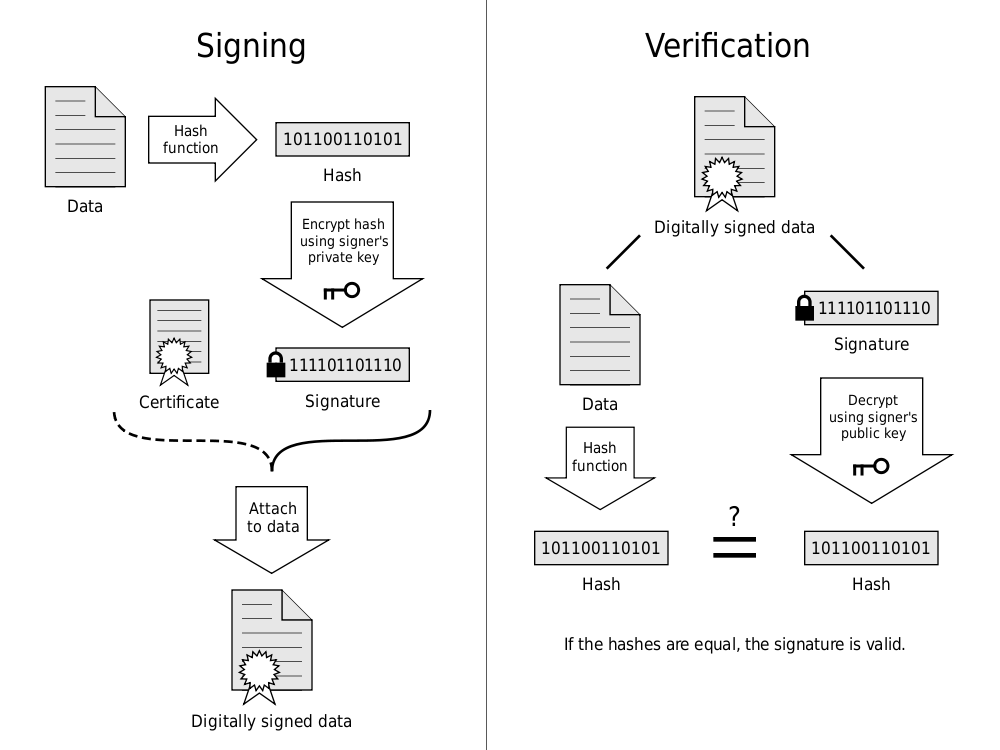
\includegraphics[width=400px]{images/signing.png}
\caption{A graphical representation of the digital signature process \cite{signing}}
\label{fig:signing}
\end{figure}


% ZKPK
\section{Zero Knowledge Proof of Knowledge}
A party might need to prove that it knows some value from time to time. Sometimes it is acceptable
to simply reveal the value, but in other cases, this might not be acceptable. For instance, imagine
if Alice, Bob, and Eve are in the same room. Victor  wants to make sure Peggy knows his phone number,
but does not want Eve to learn her phone number. Peggy cannot simply repeat Victor's phone
number, lest Eve overhear and write it down. In this case, Peggy will use what is called a
\textit{zero knowledge proof of knowledge} or ZKPK.

A ZKPK is a way to prove for one party to prove to another that it knows a secret without actually
revealing the secret. A basic use case was just described, but there are many reasons why a ZKPK
might be useful. A ZKPK can be used when there is concern that a man-in-the-middle is present
and could determine the secret (as was the case in the previous example), but to defeat this,
encryption is usually a better alternative. Where a ZKPK is very useful is when the sender does not
want to reveal the secret to the recipient. So in a similar example, say that Peggy wanted to prove to
Victor that she knew her own phone number, but did not want to give it to Victor. This is when the
use of a ZKPK is most applicable.

There are multiple different schemes that implement ZKPK behaviors. 
The scheme the author is most familiar with is called the Feige-Fiat-Shamir Identification Scheme (FFS). 
The scheme works using modular arithmetic, similar to the RSA algorithm above.
Interested readers are referred to the original paper in \cite{ffs} for more details. 

% Committments
\section{Commitment Schemes}
It is often necessary for a party to be bound to some decision it has made in the past, but without
actually revealing that decision. For example, suppose Alice and Bob are talking on the phone and
want to flip a coin to solve a dispute. This is clearly subject to much distrust, since whoever flips the
coin could lie about the result so he or she always wins.
This is where a commitment scheme would be useful.

More formally, a commitment scheme is defined as a two step procedure. In the first step, a value
is chosen and \textit{committed}. This \textit{commitment} does not reveal the value chosen, so it
may be publicly published somewhere if desired. The second step is \textit{revealing}. In this step,
the private value is revealed and then verified against the commitment previously made.

In the coin-flipping example, a commitment scheme could be employed as follows. Alice would 
secretly decide whether to call heads or tails. She would then \textit{commit} this value to Bob. Recall
that this commitment does not reveal Alice's choice. Bob would then tell Alice the result of the coin
flip. Alice would then tell Bob what she committed previously. Bob checks this value against Alice's
commitment. If the value checks out, Bob accepts that Alice actually did call that value.

Commitment schemes are fairly similar to zero knowledge proof of knowledge schemes; indeed, some
zero knowledge schemes actually employ commitments! The method the author is most familiar with
is known as Pedersen commitments. Readers interested in more details of this scheme are referred
to the original paper \cite{pedersen}.



% Describe PUFs at a general level
% Give an overview of PUF devices

\chapter{Physically Unclonable Functions}
\label{chapter:pufoverview}

\section{Comparison to Alternatives}
Here is some text

% Discuss the different PUF applications and how they relate to physical system design
% Give a general introduction to the PUF applications chapter

\chapter{Applications}
\label{chapter:applications}


% Discuss the PUF ROK and how it is relevant

\chapter{Read Once Keys}
\label{chapter:rok}

\section{Overview}
The term read-once keys (ROKs) describes the abstract notion that a cryptographic key can be read and used for encryption
and decryption only once. While it seems intuitive that a trusted piece of software could be designed that deletes a key right after
using it, such a scheme na\"{i}vely depends on the proper execution of the program. This approach could be easily
circumvented by running the code within a debugging environment that halts execution of the code before the deletion occurs.
That is, the notion of a ROK entails a stronger protection method wherein the process of reading the key 
results in its immediate destruction.

ROKs could be applied in a number of interesting scenarios. One application could be to create one-time programs~\cite{otp},
which could be beneficial for protecting the intellectual property of a piece of software. A potential client
could download a fully functional one-time program for evaluation before committing to a purchase.  A similar application
would be self-destructing email.  In that case, the sender could encrypt a message with a ROK; the message would then
be destroyed immediately after the recipient reads the message.  More generally, there is considerable interest in self-destructing
data, both commercially~\cite{ironkey} and academically~\cite{vanish}.  In addition, the use of trusted hardware tokens have been
proposed for applications including program obfuscation~\cite{obfusc}, monotonic counters~\cite{monotonictpm}, oblivious
transfer~\cite{ottamper}, and generalized secure computation~\cite{tamperhw}.  ROKs can provide the required functionality
for these applications.

Another interesting application of PUF ROKs is to defend against physical attacks on cryptographic protocols.  For example,
consider fault injection attacks on RSA~\cite{rsapub,pertrsa,insecrsa,rsaltr,fault}.  In these attacks, the algorithm is repeatedly executed
with the same key, using a controlled fault injection technique that will yield detectable differences in the output.  After enough such
iterations, the attacker is able to recover the key in full.  Similarly, ``freezing'' is another class of physical attack
that can extract a key if it was \emph{ever} stored in an accessible part of memory~\cite{freezing}.  PUF ROKs offer a unique defense against
all of these attacks because repeated execution with the same key cannot occur, and the key is \emph{never} actually present
in addressable physical memory.

The ability to generate ROKs in a controlled manner could also lead to an extension where keys can be generated and used
a multiple, but limited, number of times. For example, consider the use of ROKs to encrypt a public key {\it pk}. If an
identical ROK can be generated twice, the owner of {\it pk} could first use the key to create $e_{ROK}(pk)$ (indicating the
encryption of {\it pk} under with the ROK). Later, an authorized party could create the ROK a second time to decrypt the
key. Such a scheme could be used to delegate the authority to cryptographically sign documents.

In a sense, a ROK is an example of a program obfuscator.  An obfuscator $\mathcal{O}$ takes a program $\mathcal{P}$ as
input and returns $\mathcal{O}(\mathcal{P})$, which is functionally identical to $\mathcal{P}$ but indecipherable.  A ROK,
then, involves an obfuscator that makes only the key indecipherable.  While ROKs are promising ideals, the
disheartening fact is that program obfuscators--of which ROKs are one example--cannot be created through algorithmic
processes alone~\cite{impobf}.  Instead, trusted hardware is required to guarantee the immediate destruction of the
key~\cite{otp}.  However, we are aware of no work that has specifically undertaken the task of designing and creating such
trusted hardware for the purpose of generating a ROK.

Our insight for the design of such ``PUF ROKs'' is to incorporate the PUF in a feedback loop for a system-on-chip
(SoC) design.\footnote{Our design could also be made to work for application-specific integrated circuits (ASICs), but
we limit our discussion to SoC designs for simplicity.} That is, our design is for the PUF to reside on the same chip
as the processor core that performs the encryption. This integration of the PUF and the processor core protects the
secrecy of the key.  An attempt to read the key from memory (given physical access) will fail, because the key \emph{never
exists in addressable memory}.  Also, attempts to learn the key from bus communication will be difficult or
impossible, as each key is used to encrypt only a single message, and the key is \emph{never transmitted across the bus}.

The unpredictable nature of PUFs provides a high probability that each iteration of a ROK generation will produce a
unique, seemingly random key.  Yet, to ensure that a key can be generated to perform both encryption and decryption,
the PUF must be initialized repeatedly to some state, thus providing the same 
sequence of keys.  To accomplish this, Alice could provide an initial seed to produce a sequence of keys that are used to encrypt
a set of secrets. Alice could then reset the seed value before making the device available to Bob. Bob, then, could use the PUF to
recreate the keys in order, decrypting the secrets. As Bob has no knowledge of the seed value, he is unable to reset the
device and cannot recreate the key just used.

Astute readers will note the similarities between our approach and using a chain of cryptographic hashes to generate
keys.  That is, given a seed $x_0$, the keys would be {\sf H}$(x_0)$, {\sf H}({\sf H}($x_0$)), etc., where {\sf H}
denotes a cryptographic hash function.  The insight of our approach is that a PUF, as a trusted piece of hardware,
can provide a hardware-based implementation that is analogous to a hash function, but is more secure than
software implementations of such algorithms.
\footnote{The previous sections were taken from~\cite{PUFROK}}

\section{Read Once Keys (ROK)}
Our formal notion of a ROK is based on an adaptation of Turing machines.  Specifically, define the machine $T$ to be
\begin{center}
\begin{tabular}{c}
$T = < Q,q_0,\delta,\Gamma,\iota >$
\end{tabular}
\end{center}
where $Q$ is the set of possible states, $q_0$ is the initial state, $\delta$ defines the transition
from one state to another based on processing the symbols $\Gamma$, given input $\iota$.  Readers familiar with Turing
machines will note that $\iota$ is new.  In essence, we are dividing the traditional input symbols into code ($\Gamma$)
and data ($\iota$).  For the sake of simplicity, we assume that $\iota$ only consists of messages to be encrypted or
decrypted and ignore other types of input data.  Thus, the definition of $\delta$ is determined by the execution of
instructions $\gamma_1, \gamma_2, \ldots, \gamma_i$, where consuming $\gamma_i \in \Gamma$ results in the transition from state $q_i$ to
$q_{i+1}$.  Based on this formalism, we propose the following primitives.

\begin{itemize}
\item The \emph{\bf encrypt primitive} {\sf Enc}$(\gamma_i,q_i,m)$ encrypts the message $m \in \iota$ given the instruction
$\gamma_i$ and the state $q_i$.  The system then transitions to $q_{i+1}$ and produces the returned value as $e(m)$ as a side effect.
\item The \emph{\bf decrypt primitive} {\sf Dec}$(\gamma_j,q_j,e)$ decrypts the ciphertext $e \in \iota$ given the instruction
$\gamma_j$ and the state $q_j$.  If the decryption is successful, the primitive returns $m$.  Otherwise, the return value is 
denoted $\emptyset$.  The system then transitions to $q_{j+1}$.
\end{itemize}

Informally, $\gamma_i$ and $q_i$ describe the current instruction and the contents of memory for a single execution
of a program, and capture the state of the system just before executing the encrypt or decrypt primitive.  That is,
if the execution of the program is suspended for a brief time, $\gamma_i,q_i$ would describe a snapshot of the
stack, the value stored in the instruction pointer (IP) register, the values of all dynamically allocated
variables (\emph{i.e.,} those on the heap), etc.  In short, it would contain the full software image for that
process for that precise moment in time.  Once the program is resumed, the symbol $\gamma_i$ would be consumed, and
the system would transition to state $q_{i+1}$.  Given these primitives, we present the following definition. \\

\noindent \textbf{Definition:}  A \emph{\bf read-once key} (ROK) is a cryptographic key $\mathcal{K}$ subject
to the following conditions:
\begin{itemize}
\item Each execution of {\sf Enc}$(\gamma_i,q_i,m)$ generates a new $\mathcal{K}$ and yields a transition to a unique $q_{i+1}$.
\item The first execution of {\sf Dec}$(\gamma_j,q_j,e)$ returns $m$ and transitions to $q_{j+1}$.  All subsequent executions
return $\emptyset$ and transitions to $q_{j+1}'$, even when executing the machine $< Q,q_0,\delta,\Gamma,\iota >$ with $e$,
except with negligible probability.
\item The probability of successfully decrypting $e$ without the primitive {\sf Dec}$(\gamma_j,q_j,e)$ is less than or equal to
a security parameter $\epsilon$ ($0 < \epsilon < 1$), even when given identical initial states.  $\epsilon$ must be no
smaller than the probability of a successful attack on the cryptographic algorithms themselves.
\end{itemize}

What these definitions say is that the ROK Turing machine is non-deterministic.  Specifically, during the first execution of
a program\footnote{Observe that the program doing the encryption is separate from the one doing
the decryption.  If the encryption and decryption occurred in the same program, the decryption would succeed, as the key would
have just been dynamically generated.  In contrast, when the programs are distinct, only the first execution of the decryption
program will succeed.} that encrypts a message $m$, $\delta$ will define a transition from $q_i$ to $q_{i+1}$ based on the primitive
{\sf Enc}$(\gamma_i,q_i,m)$.  However, the second time, the key will be different, and the state transition will be from
$q_i$ to $q_{i+1}'$.  Similarly, the first execution of a program that decrypts $e(m)$ will traverse the states
$q_0, \ldots, q_j, q_{j+1}$, where $q_{j+1}$ is the state that results from a successful decryption.  However, returning
the machine to its initial state $q_0$, using the same instructions $\Gamma$, the state traversal will be $q_0, \ldots,
q_j, q_{j+1}' \ne q_{j+1}$, because the decryption fails.  Thus, ROKs incorporate some unpredictable element that does
not exist in traditional Turing machines:  the history of prior machine executions.  That is, for any given machine $T$, only
the first execution (assuming either the encrypt or decrypt primitive is executed) will use the transitions defined by $\delta$.
The second (and subsequent) executions will use $\delta'$, as the state after the primitive is invoked will differ.

Clearly, these definitions capture the intuitive notion of a ROK.  The key $\mathcal{K}$ is generated in an
on-demand fashion in order to encrypt a message.  Later, $\mathcal{K}$ can be used to decrypt the message, but only
once.  After the first decryption, the key is obliterated in some manner.  Specifically, even if the contents of
memory are returned to match the program state $\gamma_j,q_j$ as it existed before the first call to {\sf Dec}$(\gamma_j,q_j,e)$,
the decryption will fail.  The intuition here is that a special-purpose hardware structure must provide this
self-destructing property.

Observe that an adversary $\mathcal{A}$ may opt to attack the cryptographic algorithms themselves.  In such an
attack, the number of times the key $\mathcal{K}$ can be read by an authorized party is irrelevant:  $\mathcal{A}$
is never authorized.  If the cryptographic scheme is sufficiently weak, $\mathcal{A}$ may succeed in recovering
the message (or the key itself).  The ROK property offers no additional security against such an attack.  That
is, we are making no special claims of cryptographic prowess.  For this reason, we require that $\epsilon$ be no
smaller than the probability of a successful attack on the cryptographic scheme employed.

What is unique about our technique is that we are offering a means to limit the usage of a key by an authorized
party.  Clearly, with sufficient motivation, this authorized party may become an adversary himself, attempting to
recover the key $\mathcal{K}$ and subvert the system.  The parameter $\epsilon$ offers a means to specify the system's
defense against such an insider threat.  For the most sensitive data, an implementation of our design could require
a very low level of $\epsilon$, making the probability of subverting the ROK property equal to the probability of
a brute-force attack on the cryptographic algorithm.  In applications that are less sensitive (\emph{i.e.,} the
ROK property is desirable, but not critically important), $\epsilon$ could be larger.  In short, $\epsilon$ captures the
flexibility to adjust the security guarantees of the ROK according to desired implementation characteristics.
\footnote{The previous sections were taken from~\cite{PUFROK}}

\section{PUF-based ROKs}
Figure~\ref{fig:basicrok} shows a block level diagram of a basic PUF rok design. It consits of several different
components. The Processor Core (PC) is what interacts with the computer itself and the internal components of the
PUF ROK. It also handles the various input and output tasks required.
 The PC is connected to the Cryptography Core (CC), which is responsible for performing the various
cryptographic operations as well as communicating with the interal feedback loop.
The internal feedback loop consists of a register wired to the PUF which is wired to an error correciton unit, which
is then in turn wired back to the register and the CC.

The CC is a stand-alone hardware component that provides cryptographic services to the PC.  The CC provides the 
following service interface to the PC:
\begin{itemize}
\item {\sf Init}$(x_0)$ : an initialization routine that takes an input $x_0$ as a seed value for the PUF.  There is no return value.
\item {\sf Enc}$(m)$ : an encryption primitive that takes a message $m$ as input and returns the encrypted value $e(m)$.
\item {\sf Dec}$(e(m))$ : a decryption primitive that takes a ciphertext as input.  This service returns the plaintext $m$ only
on the first execution.  Subsequent calls to this service return $\emptyset$.
\end{itemize}

Upon a call to the encryption function, the PUF is executed with the contents of the register, error correction is stored,
and then the response overwrites the contents of the register. The response is also passed back to the cryptography
core where it can be used to generate an encryption key. This feedback loop ensures that once a key has been used
once, it cannot be used again, since it has been overwritten in the register.

When decryption is desired, the Init function must be used to re-seed the device so that the proper value is in the
register. Then, when Decrypt is called, the value in the register will be used as the challenge to the PUF, any errors
will be corrected by the error correction unit, and the result will overwrite the register and also be passed into the
CC. The response will then be used to derive the decryption key for the message.

\begin{figure}[!ht]
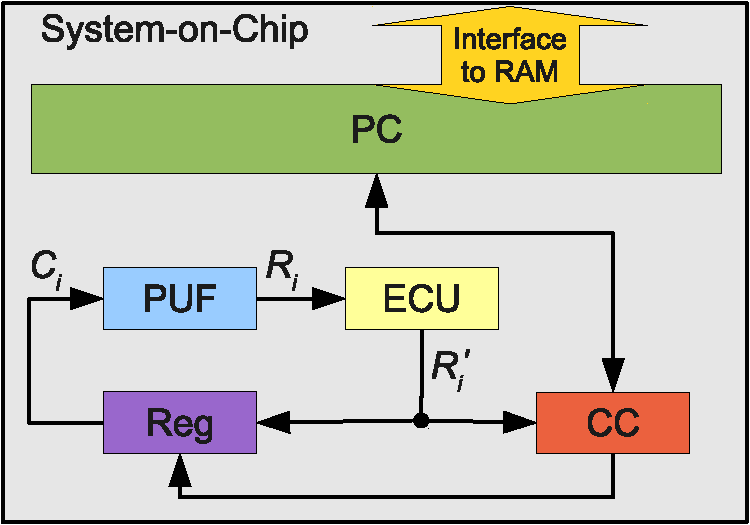
\includegraphics[width=500px]{images/rok_soc.pdf}
\label{fig:basicrok}
\caption{Block Level View of a Basic PUF ROK Device}
\end{figure}
\FloatBarrier

Note that the CC uses the error corrected PUF response to derive a key, but does not use it as a key directly.	Typically
a hash algorithm is applied to the key first. This prevents the PUF from potentially being modeled, as described in
Chapter~\ref{chapter:pufoverview}.

\subsection{PUF ROKs as a Physical System}
Because of their nature, PUF ROKs would be considered a peripheral physical system. This is because they rely
on an interaction between themselves and a computer to augment the functionality of the computer; 
they do not necessarily interact with the world just by themselves.

As a peripheral physical system, the PUF ROK must be resiliant against various types of environmental attacks, such
as freezing and power analysis, as discussed in the next section, but they also must be very aware of the
interactions they have with a host system and the dangers that can pose.

\section{Security Considerations}
For our security analysis, we consider the case of a probabilistic polynomial-time (PPT) attacker $\mathcal{A}$,
with two goals.  First, the goal of $\mathcal{A}$ is to recover just the key used to encrypt or decrypt a
single message.  The second goal considered is to model the PUF, which would enable the attacker to emulate
the PUF ROK in software, thereby negating the hardware ROK guarantee.  Initially, in both cases, we assume
the adversary is capable of (at most) eavesdropping on bus communication.  That is, the adversary is unable
to observe communication between the cores in the SoC design.

Under this model, $\mathcal{A}$ is able to observe the data passing between the PC and memory, or between
the PC and a network.  Observe, though, that these messages consist exclusively of the plaintext $m$ and the
encrypted $e(m)$.  Thus, the attack is a known-plaintext attack.  However, this information offers no
additional knowledge to $\mathcal{A}$.  Even if $\mathcal{A}$ managed to reconstruct the key $\mathcal{K}$
(with negligible probability under the PPT model), this key is never used again.

The only use of reconstructing $\mathcal{K}$ in this manner is to attempt to reverse engineer
the behavior of the PUF.  However, recall that our design involved hashing the PUF output when
creating the keys.  Consequently, $\mathcal{K}$ = {\sf H}$(R_i)$, where {\sf H} is a robust cryptographic
hash function.  As a result, $\mathcal{A}$ again has only a negligible probability of reconstructing $R_i$.
Yet, we can take this analysis even further, because $R_i$ by itself is useless.  That is, $\mathcal{A}$
would also need to know the corresponding $C_i$ (or $R_{i+1}$) to begin to model the PUF.  Thus, $\mathcal{A}$
would have to accomplish a minimum of \emph{four} feats, each of which has only a negligible probability of
occurring.  Thus, we do not find such an attack to be feasible.

To continue the analysis, we loosen our assumed restrictions and grant $\mathcal{A}$ the ability to probe
inside the SoC and observe all data transferred between the cores.  Clearly, such an adversary would
succeed, as the data passed between the PUF and the CC occurs in the open.  However, this attack model
is so extreme that only the most dedicated and motivated adversaries would undertake such a task.
Similarly, users who are faced with such powerful adversaries are likely to have extensive resources 
themselves.  Thus, these users are likely to shield the processor using known tamper-resistance
techniques, and we find this threat to be minimal.

Moving away from the PPT model, we can return to the discussion of fault
injection~\cite{rsapub,pertrsa,insecrsa,rsaltr,fault} and freezing~\cite{freezing}
attacks.  Fault injection attacks fail to threaten the confidentiality of the system,
because these attacks are based on repeatedly inducing the fault with the same key.  However, PUF ROKs can
only be used once.  At best, a fault injection would become a denial-of-service, as the key would not
correctly enrypt or decrypt the message.  Freezing attacks are similarly unsuccessful, because they operate
on the assumption that the key existed in addressable memory at some point.  However, that is not the case
with PUF ROKs.  These keys are generated dynamically and are never explicitly stored outside the processor
itself.  Thus, PUF ROKs offer robust defenses against these physical attacks.

One final class of attacks to consider is power analysis~\cite{dpa}.  Simple power analysis (SPA) involves
monitoring the system's power fluctuation to differentiate between portions of cryptographic algorithms.
This information leakage can reveal how long, for instance, a modular exponentiation takes, which reveals
information about the key itself.  Differential power analysis (DPA) observes the power fluctuations over
time by repeatedly executing the cryptographic algorithm \emph{with the targeted key}.  Ironically, DPA
is considered harder to defend against than SPA.  And yet, PUF ROKs are immune to DPA (since repeated execution
is not allowed) while vulnerable to SPA.  Even though SPA is a potential threat, known techniques can prevent
these attacks~\cite{sidechan}.\footnote{The previous sections were taken from~\cite{PUFROK}}

\section{Out of Order Execution}
One limitation of the basic PUF ROK design in~\ref{fig:basicrok} is that it does not allow out of order execution. That is,
if five messages are encrypted and then the third is requested to be decrypted, the PUF ROK must be re-seeded, the PUF
cycled twice, and then the third cycle can be used to actually perform the decryption. To decrypt the first message, the
PUF would again need to be re-seeded. 

Supposing this had to be done many times, this process would quickly become cumbersome. As such, it is desirable to
have a PUF ROK system that allows out of order execution. Figure~\ref{fig:rok} shows the block level design for a PUF
ROK that allows this out of order execution.

\begin{figure}[!ht]
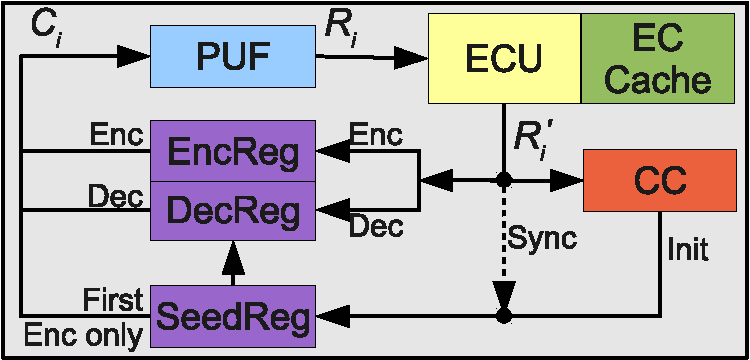
\includegraphics[width=500px]{images/rok_socreg.pdf}
\label{fig:rok}
\caption{Block Level View of a PUF ROK Allowing Out of Order Execution}
\end{figure}
\FloatBarrier

The modified PUF ROK is able to perform out of order executions by replacing the one original register with three
new registers, a seed register, an encryption register, and a decryption register. A cache is added to the error
correction unit as well. Note that all these new components are still internal to the PUF ROK design, so that no
buses are exposed externally.
The new design requires a new parameter, $N$. This parameter specifies the number of keys that will be stored in
the error correcting cache. The PUF ROK can then perform out of order execution on up to $N$ different keys.
The new design also introduces the Sync action, which is used to update the seed register and is further described
below.

Upon the initial seeding of the PUF ROK, the seed value is stored in the seed register. When the first encryption
is requested, the seed register is fed into the PUF. The response is then passed through error correction and stored
in both the error correcting cache as well as the encryption register. Note that the seed register is not updated here.
Upon request for another encryption, the contents of the encryption register will be used, rather than the seed register.

Upon a request for a decryption, if the requested key is still marked as valid in the error correcting cache,
the seed register is copied into the decryption register. The PUF is then cycled
and writes back to the decryption register enough times for the proper respone to be obtained. Note that the
error correcting unit is correcting any potential errors after each cycling of the PUF. At the conclusion of this, the
requested key is marked as used in the error correcting cache, meaning the PUF ROK will not use it again.

Because the error correcting cache has a finite amount of space, it will be necessary to clear the cache from time to
time. This is done using the Sync action. Sync is triggered when the first key in the cache has been marked as invalid.
(Note that this first key will be associated with the value currently in the seed register.) Since the values are invalid,
this means that they will never be used again, so the value in the seed register is obsolete and can be updated.
The error correction cache thus takes control of the feedback loop. It decides which key is the last used, and then cycles
the PUF, using the contents of the seed register that many times and writing the results back into the seed register.
For example, if there are 4 values stored in the cache and values 1 and 2 are invalid, the PUF will be cycled twice,
with the resulting response being written into the seed register.

\section{Implementation}
For a prototype implementation, the Saxo-L board from KNJN.com was used.~\cite{KNJN} It contains an Altera
Cyclone FPGA and an NXP LPC2132 ARM processor. The two chips are connected together by a Serial Peripheral
Interface (SPI). Additionally, a USB and a JTAG port are available, which makes for easy communication with the
various chips.

For the ease of development, we implemented only the PUF and the register on the FPGA and then implemented
the error correction unit, cryptography core, processor core, and other supporting computation on the ARM chip. 
When the PUF or register was needed, the ARM would issue a request over the SPI link to access the approprite component.
~\ref{fig:rokimpl} shows details of the implementation graphically.

\begin{figure}[!ht]
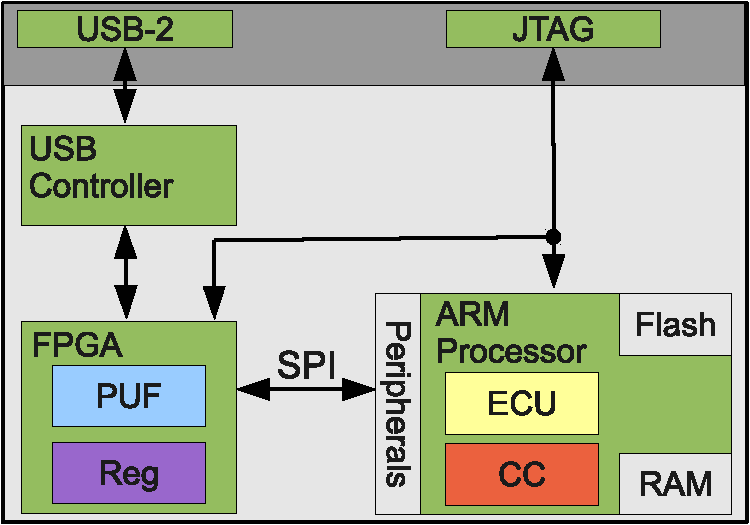
\includegraphics[width=500px]{images/rok.pdf}
\label{fig:rokimpl}
\caption{Implementation of a ROK device}
\end{figure}
\FloatBarrier

The Saxo-L board is 44 x 60 mm, which makes it very portable. A production quality device would likely be smaller.
This would allow the ROK to be implemented as a small dongle that could be plugged into a USB port potentially.

For the software portion of the project, the PolarSSL~\cite{polarssl} library was used, which is an SSL library
specifically optimized for small microprocessors, such as the LPC2132.

\subsection{Limitations}
There are some limitations to the implementation, since it is simply a prototype. The fact that the SPI bus is exposed
is a huge problem. As it currently exists, an attacker could simply attach logic probes to the bus and interecept or
modify any traffic between the FPGA and ARM chip. As such, he would be able to manipulate the values of the register
as well as what the error correction unit receives. Clearly, this is not a good thing.

This vulnerability could be mitigated by using some sort of tamper proofing, such as potting, but this is a relatively
expensive solution. Instead, the ideal solution would be to incorporate all the different components on one chip, as
shown in the original design. There are soft core ARM processors available which can be instantiated on an FPGA
already. It would be possible to simply move the entire ARM processor onto the same chip as the PUF and register.
Not only would this be more secure, but it would most likely be less expensive to manufacture a device with only
one chip, rather than two.

There are a variety of softcore microprocessors available, depending on the brand of FPGA selected, so there are
alternatives available to the ARM architecture.

\subsection{Results}
Our PUF design consisted of 32 1-bit ring oscillator PUFs, as shown in Figure~\ref{fig:puf}.
Each of these circuits consisted of a ring oscillator constructed from 37 inverting gates.
In our experiments, we found that using fewer than 37 gates yielded less consistency in the
PUF behavior.  That is, smaller PUFs increase the number of bit errors that must be corrected.
The output from the ring oscillators was linked to 20-bit
counters that were controlled by a 16-bit timer.  The timer was synchronized with a 24 MHz
clock, indicating that the timer would expire (as a result of an overflow) after 2.73 ms.
When the timer expires, the values in the counters are compared, producing a 1 or 0 depending
on which counter had the higher value.
This design used 2060 of the 2910 (71\%) logic cells available on the FPGA.  Each execution
of the PUF produced 32 bits of output.  Consequently, to generate larger keys, the ARM processor
polled the PUF multiple times, caching the result until the key size was met.

To put the performance of the PUF into perspective, we compared the execution time with measurements~\cite{nxp}
reported by NXP, the device manufacturer.  Some of NXP's measurements are reported in Figure~\ref{fig:aes}.
As each PUF execution (producing 32 bits of output) requires 2.73 ms to overflow
the timer, it is slower than encrypting one kB of data in AES.  Observe, though, that larger PUFs would
still only require 2.73 ms.  Consequently, the overhead of executing the PUF can remain small, especially
as large amounts of data are encrypted or decrypted.

\begin{figure}[ht]
\begin{center}
\begin{tabular}{l | c c l | c}
Symmetric 	& Time		& ~~~	& RSA			& Time\\
Algorithm	& (ms/kB)	& ~~~	& Operation		& (s)\\
\cline{1-2}\cline{4-5}
AES-CBC		& 1.21		& ~	& 1024-bit encrypt	& 0.01 \\
AES-ECB		& 1.14 		& ~	& 1024-bit decrypt	& 0.27 \\
3DES-CBC	& 3.07		& ~	& 2048-bit encrypt	& 0.05 \\
3DES-ECB	& 3.00		& ~	& 2048-bit decrypt	& 2.13
%RSA Operation		& Time (s) \\
%\hline
%1024-bit encrypt	& 0.01 \\
%1024-bit decrypt	& 0.27 \\
%2048-bit encrypt	& 0.05 \\
%2048-bit decrypt	& 2.13
%\end{tabular}
%\caption{RSA cryptographic measurements reported by NXP (in seconds)}
\end{tabular}
\caption{NXP cryptographic measurements}
\label{fig:aes}
\end{center}
\end{figure}

The comparison the RSA encryption and decryption is stark.  Observe that the 2.73 ms required to
execute the PUF is 27.3\% of the time to perform a 1024-bit encryption in RSA.  As the key size
increases (assuming the PUF size is increased accordingly so that only one polling is needed),
the PUF execution time becomes 0.13\% overhead for 2048-bit RSA decryption.  Thus, the performance
impact of polling the PUF during key generation is minimal.\footnote{Obviously, there is additional
work required to convert the PUF output into a usable key.  However, the precise timing of this
work is implementation-dependent, and the algorithms typically employed are significantly more
efficient than the modular exponentiation.  As such, we focus solely on the PUF measurement in
our analysis.}\footnote{The previous sections were taken from~\cite{PUFROK}}

 % PUF ROK work
% Discuss the PEAR work and how it is relevant

\section{Physically Enhanced Authentication Ring}
\label{section:pear} % PEAR work
% Discuss the DOE project and how it is relevant

\chapter{Smart Grid and Smart Meters}
\label{chapter:doe}

\section{Overview}
There has been a move recently towards the design and implementation of what is called a ``smart grid." A smart
grid is an electrical power grid which can gather information about the meters, houses, and consumers of
electricity that are attached to it.


By gathering information from a smart grid, a power company can more efficiently manage its production and delivery
of electricity, thus reducing cost. Not only does the smart grid help the power company, but by providing analytics to
its customers, customers can adjust their consumption habits to lower their bills as well. With the increasing cost of
fossil fuels and the increasing energy consumption of today's consumer, reducing wasted electricity will be very useful.

Naturally, with this increase in functionality, there is an increase of risk as well. While the power company can use
the smart grid to smartly redirect power to where it is needed, an attacker might try to direct power away from an
area or direct so much power to an area that the system becomes overloaded and fails.

As a response to the increased dangers that a smart grid provides, we describe a system that is designed to allow
for secure, yet convenient, communication and management between consumers and the utility company. Existing
systems are leveraged, such as the ZigBee mesh network~\cite{zigbee}, which is further described below.
One of the main things that is critical in this new system is that individual meters are able to be uniquely identified
so billing can be done correctly, but also so no one can impersonate them. This is a perfect opportunity for PUF
technology.

\section{Actors}
For the rest of the chapter, it will be useful to discuss the different players in the smart grid scenario.

\subsection{Utility Company}
One of the major players in the smart grid scenario is the utility company. The utility company is responsible for
generation of the electricity using techniques such as coal power, hydroelectric, wind, among others. The utility
company is also responsible for managing the dynamic delivery of power to areas that need it.

Finally, the utility company is also responsible for maintaining information on all of its customers and billing them
appropriately.

\subsection{Substations}
Substations receive large amounts of high voltage power from the utility company. However, this power is not ready
for end user consumption. The substation thus takes the power from and converts it to  more reasonable levels
that is suitable for being to delivered to end users.

The substation will communicate with the utility company to tell the utility how much load it is under. Depending on
the load, it will then receive more or less power. It also acts as a sort of ``collector" node for different smart meters.
Smart meters will communicate with the substation which will then relay the data back to the utility company.

\subsection{Smart Meters}
A smart meter is much like a regular power meter but with some added features. Smart meters measure power as
a normal meter, but they can typically be configured so that they can also ``rewind" if a user is pumping power back
into the grid. Additionally, smart meters have many different features which allow real time information and analytics
about power consumption to be obtained.

One of the large benefits of smart meters is that the utility company can communicate and read them without
necessarily sending a worker out to read the values. This is much faster and more cost effective than traditional
power meters. This is accomplished using some sort of wireless interface. Typically, the ZigBee~\cite{zigbee}
~\cite{aminetworking}
wireless protocol is used and is set up so that all meters form a mesh network with each other. This allows meters
that are not within wireless range of a substation (or some other communication center) to still talk to the substation.
This is accomplished since each smart meter not only transmits its own data, but it also acts as a relay for other nodes
in the mesh network.

Note that smart meters have some amount of general purpose computation, but they are not very powerful. As such,
it is necessary to optimize programs so that they can be run on the smart meters.

The smart meters used in this project are produced by Landis+Gyr. They consist of two components of interest. One
board is called the ``metering board" and is responsible for measuring and recording information about the actual
power consumption of attached devices. The other board is called the ``communication board". It is responsible for
performing the different types of communication as necessary. The two are connected over an event-based interface,
but this interface is not encrypted. 

There are 5 security levels on the smart meter, each giving a different amount of privilege to different meter controls,
with level 0 being read only access and level 5 giving control of everything. There is a table in the smart meter which
stores each of the corresponding keys for the levels; These keys are referred to as access level keys.
Communication between the utility and smart meter is encrypted
using a random session key, which is derived from an encryption key.

\section{Physical Systems}
The actors above are clearly examples of physical systems. All three heavily interact with the environment around them
to fulfill the power needs of consumers.

The utility company as a whole might not be considered a physical system, but parts of it will definitely be considered
examples of deployed physical systems. The utility must manage the production of electricity by its generators as well
as well as manage the communication of commands to the various smart meters, via the mesh network.

Substations could also be considered deployed physical systems, since they perform a large amount of interaction
with the physical world to transform the power from the utility company into power that is usable by consumers.
They additionally must take a large amount of input from both consumer smart meters and the utility to decide how
to manage the power resources in a dynamic way.

The smart meters are deployed physical systems. A large part of the smart meters job is to record and analyze
the power usage of the home or building they are attached to. This requires interaction with the physical world. However,
smart meters are also clearly networked, since they can have so much interaction across them (in the 
concept of the mesh network) and the utility company.

\section{Protocol}
Our goal is to provide a protocol that allows for secure, authenticated communication between the utility company and
smart meters, in the presence of and despite different types of adversaries.
We leverage the use of a PUF device in conjunction with the smart meter to uniquely identify the smart meter to the
utility company.

Before describing the protocol itself, it will be helpful to discuss the information each party is expected to maintain.
The utility company will maintain a database containing two tables, one for zero knowledge commitments and the 
other for 
access level keys. The first table, referred to as the authentication table, will correlate a specific meter with a zero knowledge proof.
The second table, referred to as the access level key table, will correlate a smart meter with the five keys for the five different security levels of the 
meter. This table also stores the encryption key.

The smart meter needs to store the public key of the utility company and also maintain a ``master key"
that is generated internally using the PUF. 

Both parties also need enough information about
the mesh network to ensure that they can communicate with each other. Both parties also need to share the
encryption key, which is used to derive temporary session keys.

The first step that must be done is that the utility company must record a zero-knowledge commitment from the 
smart meter for a specific challenge. This is illustrated in Figure~\ref{fig:doeconfig}. This step is required so that later
in the protocol, the smart meter can execute a zero-knowledge proof to prove its identity.
Note that this step must be done out-of-band from the mesh network, lest an adversary enter an invalid commitment.
This could be done at manufacture time or at installation time by a technician, as long as it is executed through a secure channel.

\begin{figure}[!ht]
\centering
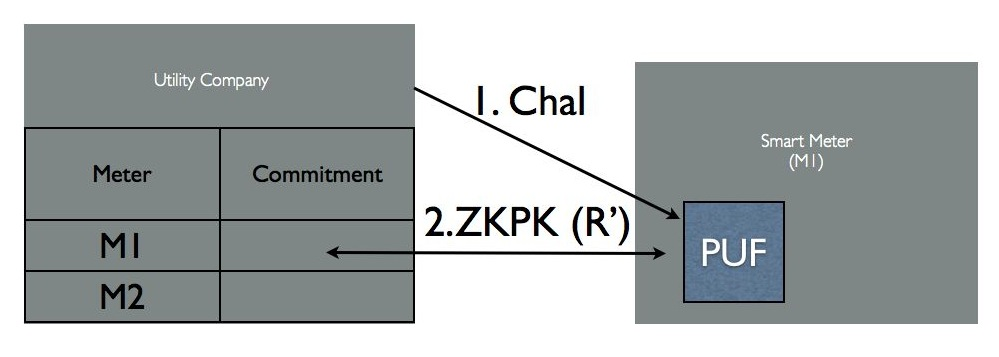
\includegraphics[width=400px]{images/doe_auth_config.jpg}
\caption{Enrollment of the commitment}
\label{fig:doeconfig}
\vspace{-20pt}
\end{figure}
\FloatBarrier

After the commitment phase has been completed and the meter has been deployed, the \textit{keying} operation
can be performed. This operation starts by executing a key derivation protocol. Recall that the smart meter 
maintains a ``master key" which is generated by the PUF. 
This master key is passed through some sort of one-way function, such as a hash
in the style of $K_1=H(MK|1), K_2=H(MK|2)...$ so that six new keys are derived, but the original master key is
never revealed. These six keys are then
encrypted under the public key of the utility company. All the encrypted keys as well as a zero knowledge proof
are then sent to the utility company. The ZKPK allows the utility company to authenticate the encrypted keys before
updating its database with the six new entries. This transmission step is detailed graphically in~\ref{fig:doeusage}.
Figure~\ref{fig:keyderivation} graphically describes the key derivation process.

Note that the PUF uses an internal feedback loop, so that every invocation of the keying procedure will generate a
different PUF response, which will in turn generate different derived keys.

\begin{figure}[!ht]
\centering
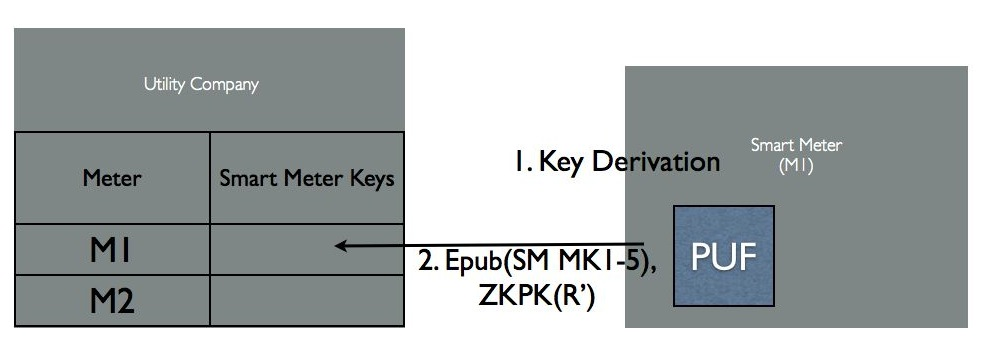
\includegraphics[width=400px]{images/doe_key_config.jpg}
\caption{Storage of the derived keys}
\label{fig:doeusage}
\vspace{-20pt}
\end{figure}
\FloatBarrier

\begin{figure}[!ht]
\centering
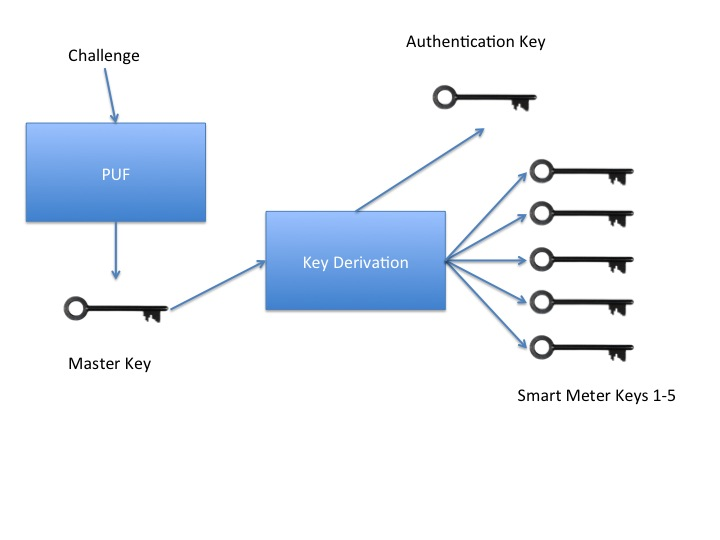
\includegraphics[width=400px]{images/keyderivation.jpg}
\caption{The key derivation process}
\label{fig:keyderivation}
\vspace{-25pt}
\end{figure}
\FloatBarrier


After the utility company has received these five access level keys and the encryption key, 
interactions between the smart meter and the utility company
will then proceed as it currently does. That is, the smart meter and utility company will use the shared encryption
key to compute a temporary, symmetric session key which will be used to encrypt data that is sent between the two.

Note that since the smart meter has limited computation powers, the operations above are fairly expensive. This
is acceptable though, since the enrollment and keying operations will be done very infrequently. If they need to
be re-run, this can be planned ahead for off peak times, such as in early morning and consumers can be notified
of this. The symmetric session key is frequently used, but symmetric encryption is much less computationally expensive
than asymmetric encryption.

Additionally, note that the utility company signs any correspondence during the enrollment or keying stages.
This allows the smart meter to validate the signature and thus ensure that commands are actually coming
from the utility company.

\section{Security Considerations}
Because there are several different ways in which the system could be compromised and the gravity that
such a compromise could have, it is necessary to consider and discuss the different security issues. 

Note that a distinction is made between the set of initial enrollment and keying operations that we defined versus
the existing system of encryption using session keys.

\subsection{Meshnet Transmission Security}
% Discuss how we use application level security, not just the ZigBee and other protocols
One potential problem is that when data is being transmitted across the meshnet, rather than relaying, a node
may attempt to read the data in transit. This would be considered a man in the middle attack. There are encryption
layers imposed by the ZigBee protocol and other transmission protocols, but it stands to reason that if a node were
malicious, it might be able to crack these layers.

As such, we add another layer of security at the application layer. Data is encrypted under the public key of the utility
company during the keying operation. As such, an adversary would be required to compromise the public key
algorithm, which is considered computationally unfeasible. A more likely attack would be to compromise the private key
of the utility company. This possibility is considered separately below.

Data being transmitted using the session key between the utility company and smart meter is encrypted under a
symmetric key algorithm, EAX', which is a variant of AES that is defined under ANSI standard 
C12.22~\cite{ansi1222}~\cite{eax}. As such, an adversary would have to be able to defeat this algorithm to make
any progress. An attack on EAX' has been reported~\cite{eaxflaw}, but this attack is new and may not be effective
enough to compromise the total integrity of the communication.

The system is also resilient against replay attacks in this situation, since both time stamps and nonces are incorporated.
As such, any replay will have invalid time stamps and nonces, so will not be valid.

There is a risk of a denial of service if an active adversary simply drops all traffic, but this is considered an acceptable
risk.

\subsection{Compromised Smart Meter Key or Encryption Key Compromise}
It is possible that somehow, one of the five smart meter keys or the encryption key used to derive session keys
could be compromised. This might happen if an employee copies a key from the database or for any other number
of reasons. Even if this happens, security is only temporarily effected.

Recall that the master key generated from the PUF is passed through a one way, key derivation process. As such,
even if one of the derived keys (the smart meter keys or the authentication key) is compromised, the master key
is still secure. To re-secure the system, the keying procedure will then be re-run, which will provide a brand new set
of smart meter keys and authentication key.

This procedure is essentially analogous to a re-key request, even if there is no compromise.

Note that this case is separate from the databases containing this information, which is considered below.

\subsection{Utility Database Compromise - Commitment Table}
If the commitment table in the utility database is compromised, the results will not be catastrophic. Since the committed
values for the ZKPK do not leak any information, the adversary will not be able to impersonate any users or garner
any new information about the underlying authentication key.

The worst case is when the adversary changes the committed values in the database. This would essentially create a
denial of service attack. However, he could also update the database with his own commitment value and place
himself between the smart meter and the utility company as an active MITM and then impersonate the smart
meter. 

Since he would be able to authenticate to the utility server, he could thus send false data about consumption or 
whatever he wanted. This threat could be dealt with by making sure that the database is very secure
and that the entries are  carefully monitored and updates are only allowed during the keying operation.

Note that in this case, the adversary would not be able to impersonate the utility company to the smart meter,
since he would not know the private key of the utility, which is necessary to sign the various messages.

This compromise would have no effect on the messages being sent under the temporary session key, since
there is no need for the authentication key during that stage.

\subsection{Utility Database Compromise - Key Tables }
It is possible that the database storing the smart meter access level keys or encryption key could be compromised. 
If these keys were compromised, the adversary could then access the sensitive commands
of the smart meter or read the interim traffic between the two parties.

However, this is not necessarily a real danger, since the keys are encrypted under the utility's private key before being
stored into the database. As such, the adversary would only recover ciphertext. Assuming he cannot break the public
key algorithm, the data will remain secure.

There is a possibility that if the database was compromised, the adversary might have been able to recover a key
as it is being decrypted in memory and record that. As such, it is wise to execute a re-keying operation for any meters
whose information was stored in that database.

\subsection{Utility Company Private Key Compromise}
One of the worst case scenarios is that the private key of the utility would become compromised. As previously
described, the smart meter's PUF-derived master key would remain secure, since it is never transmitted.

However, all smart meter access level keys and encryption keys could potentially be compromised, since the adversary
would record all traffic during the keying operation and use the private key to recover the keys.

Once those keys were recovered, it would be trivial for the adversary to communicate with the smart meter to
execute sensitive commands, request re-key operations, or whatever the adversary desired.

To recover from this attack, the old private key would first need to be discarded. Following that, the new public key would
need to be installed in every single meter in the grid. This would have to be done by hand, since any network
transmissions could not be trusted. Additionally, every smart meter would then need to execute the keying operation
so that the utility company could then update its database with the new values.

These recovery procedures would be very expensive and time consuming. As such, it is critical that the private key
never becomes compromised. Key management is a difficult, open problem that needs to be solved.

\subsection{Smart Meter Physical Security}
Since smart meters are physical systems, it is necessary to discuss and consider some of the physical threats they face.

The smart meters are actually designed to be fairly tamper resistant. If the external glass shell is removed without the
use of a technician's key, a signal is sent over the network to alert the utility company. After that happens, the utility
company can then flag any future traffic as suspicious and send a technician out to investigate and fix the meter.
Regardless, improving the tamper resistance of smart meters would be a good step to take.

Because the smart meter is doing cryptographic operations, it could potentially be vulnerable to power analysis
attacks as well as monitoring of emitted signals. To resolve this, some sort of potting mechanism, power filtering,
and shielding should be implemented. 

As previously described, the PUF is extremely resilient against tampering, so it will likely not be a problem.
Incorporating all the different components on a system on chip will be a good step towards security, since this will
hide all the internal buses as well as protect the areas with sensitive information stored on them.

\section{Implementation}
For the proposed scenario and protocol, we developed a proof of concept implementation. In the interest of time and
difficulty, rather than creating an entire smart meter from scratch, we opted to implement the 
PUF inside an FPGA and perform some of the network communication and computations on a PC, the smart meter
PC, which was connected to another PC, which is modeling the utility company. The smart meter PC is connected
to an actual smart meter via an optical port. The smart meter is also connected to the utility PC via a ZigBee interface,
as would be used in the actual field. Figure~\ref{fig:doeimpl} represents the prototype architecture.

\begin{figure}[!ht]
\centering
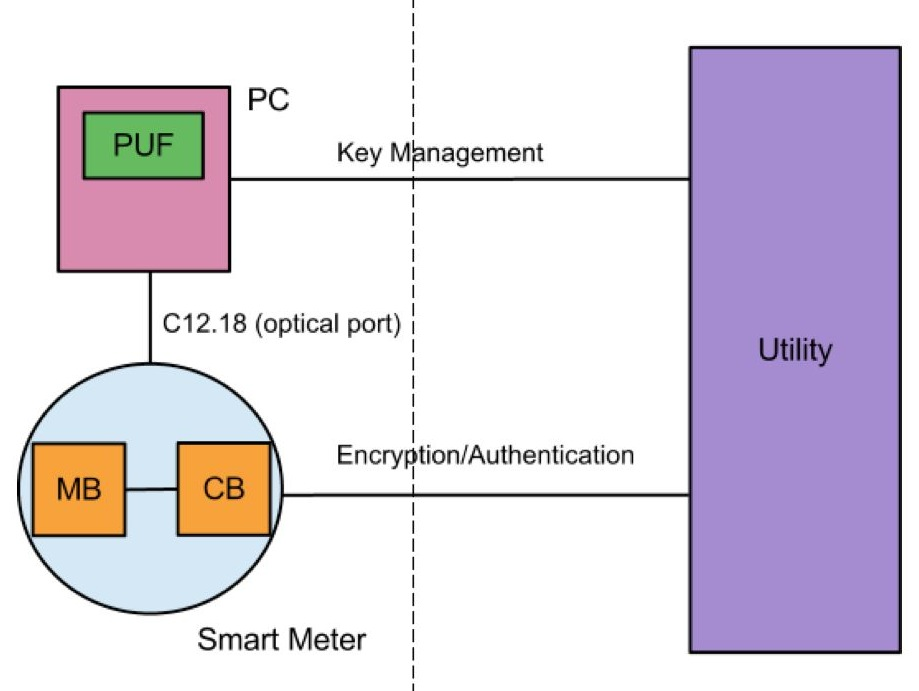
\includegraphics[width=400px]{images/doe_impl.jpg}
\caption{Prototype implementation of smart grid project}
\label{fig:doeimpl}
\vspace{-25pt}
\end{figure}
\FloatBarrier

We used the Xilinx Spartan-6 Embedded Development board for our FPGA platform. This board was useful since we 
were able to incorporate an existing PUF design on it. Additionally, we were able to use the Microblaze soft core
microprocessor which Xilinx provides. As mentioned in Chapter~\ref{chapter:pear} and Chapter~\ref{chapter:rok},
it is a good idea to include the microprocessor on the same chip as the PUF device. This allows buses sending
sensitive information, such as PUF responses, to be better protected against adversaries. Again, inserting logic
probes into the inner parts of the chip would most likely disrupt the PUF, so any results obtained about the PUF would
thus be useless.

For the smart meter PC, we created an application in C++ which uses standard networking libraries to communicate
with the utility PC. The smart meter PC interacts with the PUF board via a serial port connection. The PC also contains
drivers and code to communicate with the actual smart meter over an optical port interface.

\subsection{Limitations}
Our approach has many different components that are not necessarily going to be present in an actual, deployed
system. For instance, the fact that the PUF board and the smart meter PC are separate from the smart meter is
a major issue that would not work in the field. 

In the future, it would be better to integrate all the control circuitry,
PUF device, and metering circuitry into a single chip, such as a large FPGA or even an ASIC design. In this way, only
one chip would need to be installed into the smart meter, rather than the large amount of devices currently needed.
 % DOE work

% Summary and/or conclusions are optional but often used.
% The summary and/or conclusions often are the last
% major division(s) of the text.
% Reference: TM 32.
% CHANGE NEXT LINE?
%
%  summary.tex  2007-02-06  Mark Senn  http://www.ecn.purdue.edu/~mark
%

\chapter{Summary}
\label{chapter:conclusion}

Systems that interact with the physical world are not only becoming more pervasive, but also more powerful
from a computing perspective. It is helpful to classify these systems into groups of standalone, deployed, and
peripheral physical systems. The distinction lies in how they communicate with other systems,
such as the ones connected over the internet.

There are many different security issues facing physical systems. Not only must they compensate for threats similar
to those faced in software, such as impersonations, man-in-the-middles, and replay attacks, they must also
contend with threats specific to a system that exists in the physical world. These include power analysis attacks,
which can glean information from power consumption, signal injection attacks, which can alter system behavior by
bombarding the system with wireless signals, and simple tampering, such as breaking components or attaching logic
probes.

The technology of Physically Unclonable Function (PUF) was presented, which allows strong guarantees of device authenticity
to be made by leveraging the challenge-response properties of PUF. These devices are able to offer these guarantees
since they cannot be duplicated using a manufacturing process, so the responses they give to given challenges are
always distinct from other PUFs. PUFs require a certain amount of support circuitry to deal with bit errors that occasionally
occur, but this is acceptable and solvable using existing error correction techniques.

It is possible to utilize PUF devices in conjunction with certain cryptographic protocols, such as zero knowledge proof
of knowledge (ZKPK) proofs, to implement interesting applications. Several different applications were presented, each of
which demonstrated the use of PUF in a different context.

The PUF ROK application leveraged a PUF device to create keys that, once used, are unrecoverable. This was done by
giving the PUF an initial ``seed" value and then creating a feedback loop with the PUF. When the PUF generated a response,
it would overwrite the previously stored value. Since PUFs are one-way functions, there is no way to go backwards and
recover the value that was previously used. These ROKs could then be used to create ``self-destructing" documents
or for an authority to give a delegate a limited number of a higher privilege level.

The PEAR application used PUFs in a way to uniquely and securely identify devices, despite insecure communication
channels. In addition to a PUF, a ZKPK protocol was used to provide this benefit. The PUF as well as an external keypad
make up a PEAR device so that data can be entered securely. The initial goal was to allow users to be able to log in
to websites securely, even if a hardware key logger was attached to the keyboard. This is possible, but PEAR also
allows this capability in the presence of software threats on the PC, since all traffic is encrypted.

Finally, the smart grid project utilized PUFs to provide strong guarantees of smart meters' identity. This is critical
because if the utility company was not sure of meters it was communicating with, catastrophic attacks would be possible,
such as overloading of power handling circuits. The PUF was again used in conjunction with ZKPK proofs to
protect information in transit between the two parties. Additionally, since the utility company is required to maintain
a large database, storing ZKPK commitments, rather than secrets directly, is a much more secure approach. Another
interesting point of this application was that the PUF generated and maintained a master key internally, 
but derived keys were used in all steps of the protocol. This protects the long term security of the device, even in the 
event of certain security compromises.

These different applications show the versatility of PUF technology in helping to secure physical systems.
Depending on which cryptographic tools and protocols they are used in conjunction with, PUFs can be used
in a variety of different ways, as was demonstrated.

% Recommendations are optional.
% You may include recommendations as a major division if your
% subject matter and research dictate.
% Reference: TM 32.
% CHANGE NEXT LINE?
%%
%  recommendations.tex  2007-02-06  Mark Senn  http://www.ecn.purdue.edu/~mark
%

\chapter{Recommendations}

Buy low.  Sell high.


% Appendices are optional.
% Appendices are not necessarily part of every thesis. Appendices are used
% for supplementary illustrative material, original data, computer programs,
% and other material not necessarily appropriate for inclusion within the
% text of your thesis. 
% Reference: TM 33.
% Use "\appendix" for one appendix or "\appendices" for more than one
% appendix.
% CHANGE NEXT 7 LINES?
\appendices
%%
%  revised  demo-citations.tex  2011-09-02  Mark Senn  http://www.ecn.purdue.edu/~mark
%  created  demo-citations.tex  2007-03-21  Mark Senn  http://www.ecn.purdue.edu/~mark
%


\chapter{Demonstrate Citations}

I typed

\begin{verbatim}
    For \LaTeX\ answers I refer to
    % note to self: {\em \LaTeX: A Document Preparation System\/}
    \cite{Lamport:1994}
    and then to
    % note to self: {\em The \LaTeX\ Companion\/}
    \cite{Goossens:1994}
    or
    % note to self: {\em A Guide to LaTeX\/} (1999)
    \cite{Kopka:1999}.
    % note to self: {\em A Guide to LaTeX\/} (1999)
    \cite{Kopka:1999}
    is an updated edition of the 1995 edition
    \cite{Kopka:1995}.
\end{verbatim}

to get

\begin{quotation}
    For \LaTeX\ answers I refer to
    % note to self: {\em \LaTeX: A Document Preparation System\/}
    \cite{Lamport:1994}
    and then to
    % note to self: {\em The \LaTeX\ Companion\/}
    \cite{Goossens:1994}
    or
    % note to self: {\em A Guide to LaTeX\/} (1999)
    \cite{Kopka:1999}.
    % note to self: {\em A Guide to LaTeX\/} (1999)
    \cite{Kopka:1999}
    is an updated edition of the 1995 edition
    \cite{Kopka:1995}.
\end{quotation}

%%
%  demo-figures.tex  2009-10-30  Mark Senn  http://engineering.purdue.edu/~mark
%
%  Demonstrate how to do figures.
%

\chapter{Demonstrate Figures}

The
\verb+h+
specifier used in all the examples below
tells \LaTeX\ to put the figure
``here''
instead of trying
to find a good spot
at the top or bottom of a page.
Specifiers can be combined, for example,
``\verb+\begin{figure}[htbp!]+''.

The complete list of specifiers:

\begin{center}
    \renewcommand{\baselinestretch}{1}\normalsize
    \begin{tabular}{ll}
        \bf Specifier& \bf Description\cr
        \tt b& bottom of page\cr
        \tt h& here on page\cr
        \tt p& on separate page of figures\cr
        \tt t& top of page\cr
        \tt !& try hard to put figure as early as possible\cr
    \end{tabular}
\end{center}

Label ``fi:not-centered'' is ``\ref{fi:not-centered}''.
Label ``sf:four-parts-c'' is ``\ref{sf:four-parts-c}''.

\Repeat{This is the first paragraph.}{5}

\begin{figure}[h]
  \includegraphics{plot.eps}
  \caption{%
    By default figures are not centered.
    This is a long caption to demonstrate that captions are single spaced.
  }
  \label{fi:not-centered}
\end{figure}

\Repeat{This is the second paragraph.}{10}

\begin{figure}[h]
  \centering
  \includegraphics{plot.eps}
  \caption{Use {\tt \char'134centering\/} to center figures.}
  \label{fi:centered}
\end{figure}

\Repeat{This is the third paragraph.}{15}

\begin{figure}[h]
  \centering
  \includegraphics{plot.eps}
  \caption{This is another figuure.}
  \label{fi:another}
\end{figure}

\Repeat{This is the fourth paragraph.}{10}

\begin{figure}[h]
  \centering 
  \subfigure[First subcaption.]{\label{sf:two-parts-a}  \includegraphics[width=0.3\textwidth]{plot.eps}}%
  \hskip 0.5truein
  \subfigure[Second subcaption.]{\label{sf:two-parts-b}\includegraphics[width=0.3\textwidth]{plot.eps}}
  \caption{This figure has two parts.}
  \label{fi:two-parts}
\end{figure}

\Repeat{This is the fifth paragraph.}{10}

\begin{figure}[h]
  \centering
  \subfigure[First subcaption.]{\label{sf:four-parts-a}  \includegraphics[width=0.3\textwidth]{plot.eps}}%
  \hskip 0.5truein
  \subfigure[Second subcaption.]{\label{sf:four-parts-b}\includegraphics[width=0.3\textwidth]{plot.eps}}
  \subfigure[Third subcaption.]{\label{sf:four-parts-c}\includegraphics[width=0.3\textwidth]{plot.eps}}%
  \hskip 0.5truein
  \subfigure[Fourth subcaption.]{\label{sf:four-parts-d}\includegraphics[width=0.3\textwidth]{plot.eps}}
  \caption{This figure has four parts.}
  \label{fi:four-parts}
\end{figure}

\Repeat{This is the sixth paragraph.}{10}

%%
%  THIS FILE DOES SOME UNUSUAL THINGS TO MAKE
%  IT EASIER TO DO DEMONSTRATIONS.  IT SHOULD
%  NOT BE USED AS AN EXAMPLE OF HOW TO PREPARE
%  A FILE.  SEE THE OUTPUT OF THIS FOR LATEX
%  INPUT AND OUTPUT EXAMPLES.
%




%
%  demo-mathematics.tex  2008-12-09  Mark Senn  http://engineering.purdue.edu/~mark
%

\chapter{Demonstrate Mathematics}

    % Use single spacing.
    \Baselinestretch{1}

    % You don't normally need this.
    \mbox{}

    \begin{verbatim}
% From _More Math Into LaTeX_, 4th Edition, page 152:
%     TeX uses $$ to open and close a displayed math environment.
%     In LaTeX, this may occassionally cause problems.  Don't do it.
\[
    E = mc^2
\]
    \end{verbatim}
% From _More Math Into LaTeX_, 4th Edition, page 152:
%     TeX uses $$ to open and close a displayed math environment.
%     In LaTeX, this may occassionally cause problems.  Don't do it.
\[
    E = mc^2
\]
    \vskip\baselineskip
    \hrule
    \vskip0.5\baselineskip
    \filbreak

    \begin{verbatim}
\begin{equation}
    E = mc^2
\end{equation}
    \end{verbatim}
\begin{equation}
    E = mc^2
\end{equation}
    \vskip\baselineskip
    \hrule
    \vskip0.5\baselineskip
    \filbreak

    \begin{verbatim}
% Mydefs.tex defines \be to be \begin{equation} and
% \ee to be \end{equation}.
\be
    E = mc^2
\ee
    \end{verbatim}
% Mydefs.tex defines \be to be \begin{equation} and
% \ee to be \end{equation}.
\be
    E = mc^2
\ee
    \vskip\baselineskip
    \hrule
    \vskip0.5\baselineskip
    \filbreak

    \begin{verbatim}
\be
    x = -\frac{b}{2a} \pm \frac{\sqrt{b^2 - 4ac}}{2a}
\ee
    \end{verbatim}
\be
    x = -\frac{b}{2a} \pm \frac{\sqrt{b^2 - 4ac}}{2a}
\ee
    \vskip\baselineskip
    \hrule
    \vskip0.5\baselineskip
    \filbreak

    \begin{verbatim}
% requires \usepackage{amsmath}; use align* for no equation number
\begin{align}
    a = {}& b + c\\
    x = {}& y + z
\end{align}
    \end{verbatim}
% requires \usepackage{amsmath}; use align* for no equation number
\begin{align}
    a = {}& b + c\\
    x = {}& y + z
\end{align}
    \vskip\baselineskip
    \hrule
    \vskip0.5\baselineskip
    \filbreak

    \begin{verbatim}
\[
    Z = \left(
        \begin{array}{cc}
            a& b\\
            c& d
        \end{array}
    \right)
\]
    \end{verbatim}
\[
    Z = \left(
        \begin{array}{cc}
            a& b\\
            c& d
        \end{array}
    \right)
\]
    \vskip\baselineskip
    \hrule
    \vskip0.5\baselineskip
    \filbreak

    \begin{verbatim}
\begin{equation}
    \begin{split}
        a = {}& b + c\\
            {}& + d + e
    \end{split}      
\end{equation}
    \end{verbatim}
\begin{equation}
    \begin{split}
        a = {}& b + c\\
            {}& + d + e
    \end{split}      
\end{equation}
    \vskip\baselineskip
    \hrule
    \vskip0.5\baselineskip
    \filbreak

    \begin{verbatim}
\be
    (\cos x)^2 + (\sin x)^2 = 1
\ee
    \end{verbatim}
\be
    (\cos x)^2 + (\sin x)^2 = 1
\ee
    \vskip\baselineskip
    \hrule
    \vskip0.5\baselineskip
    \filbreak

    \begin{verbatim}
If $X = \cos x$ and $Y = \sin x$ then $X^2 + Y^2 = 1$.
    \end{verbatim}
If $X = \cos x$ and $Y = \sin x$ then $X^2 + Y^2 = 1$.
    \vskip\baselineskip
    \hrule
    \vskip0.5\baselineskip
    \filbreak

%%
%  demo-multicols.tex  2007-03-19  Mark Senn  http://www.ecn.purdue.edu/~mark
%
%  Demonstrate multicols.
%
%  The multicols package must be loaded for this to work.
%  To load the multicols package put
%      \usepackage{multicols}
%  between the "\documentclass" and "\begin{document}" commands.
%

\chapter{Demonstrate Multicols}

% Put this amount of space between the columns.
\setlength{\columnsep}{0.5truein}

% Separate the columns with a vertical rule this wide.
\setlength{\columnseprule}{0.4pt}

\Repeat{This is one column.}{25}

\begin{multicols}{2}
\Repeat{This is two columns.}{25}
\end{multicols}

\begin{multicols}{3}
\Repeat{This is three columns.}{25}
\end{multicols}

\begin{multicols}{4}
\Repeat{This is four columns.}{25}
\end{multicols}

\begin{multicols}{5}
\Repeat{This is five columns.}{25}
\end{multicols}

%%
%  demo-tables.tex  2009-09-29  Mark Senn  http://engineering.purdue.edu/~mark
%
%  Demonstrate how to do tables.
%

\chapter{Demonstrate Tables}

\begin{tabular}{ll}
    \bf Label& \bf Number\\
    ta:text-only& \ref{ta:text-only}\\
    ta:fruit&     \ref{ta:fruit}
\end{tabular}

\newlength{\ta}
\newlength{\tb}
\newlength{\tc}

\settowidth{\ta}{\vbox{\hbox{Money}\hbox{Market}}}
\settowidth{\tb}{\vbox{\hbox{Stocks}\hbox{and}\hbox{Bonds}}}
\settowidth{\tc}{\vbox{\hbox{Money}\hbox{Market}\hbox{and}\hbox{Stocks}}}

%{\renewcommand{\baselinestretch}{1}
%  \begin{table}
%    \caption{%
%      \hfil Allocation of the IRA and Keogh Wealth\hfil\break
%      \mbox{}\hfil for Investors With or Without Brokerage Accounts\hfil
%    }
%    \label{tab:ira}
%    \begin{center}
%      \begin{tabular}%
%        {%
%          |%
%          c%
%          |%
%          >{\centering\hspace{0pt}}m{\the\ta}%  Money Market
%          |%
%          c%                                    Stocks 
%          |%
%          c%                                    Bonds
%          |%
%          c%                                    Diversified
%          |%
%          >{\centering\hspace{0pt}}m{\the\tb}%  Stocks and Bonds
%          |%
%          >{\centering\hspace{0pt}}m{\the\tc}%  Money Market and Stocks
%          |%
%          c%                                    Others
%          |%
%        }
%        \hline
%        IMP&
%          Money Market&
%          Stocks&
%          Bonds&
%          Diversified&
%          Stocks and Bonds&
%          Money Market and Stocks&
%          Others\tabularnewline
%        \hline
%        1& 14.19\%& 57.71\%& 12.21\%& 4.50\%& 7.36\%& 3.04\%& 0.99\%\tabularnewline \hline
%        2& 14.08\%& 58.18\%& 12.32\%& 4.44\%& 7.30\%& 2.80\%& 0.88\%\tabularnewline \hline
%        3 &14.26\%& 58.09\%& 12.27\%& 4.50\%& 7.19\%& 2.75\%& 0.94\%\tabularnewline \hline
%        4 &13.94\%& 58.11\%& 12.14\%& 4.78\%& 7.35\%& 2.68\%& 0.99\%\tabularnewline \hline
%        5 &13.92\%& 58.13\%& 11.93\%& 4.56\%& 7.60\%& 2.98\%& 0.88\%\tabularnewline \hline
%      \end{tabular}
%    \end{center}
%    This table presents the allocations of the wealth in the IRA
%    and Keogh accounts in various asset classes.
%    Results from each set of imputed data are presented here.
%    The first column lists the number of the imputations,
%    and rest of the columns lists various allocations.
%    Entrees under each asset class show the percentage of investors
%    who have most of their IRA
%    and Keogh wealth invested in that particular asset class.
%    The asset class Diversified
%    includes stocks,
%    bonds,
%    and money market investments.
%    The asset class Others
%    include investments in various life insurance products,
%    annuities,
%    real estate, etc.
%    \medskip
%    \footnotesize SOURCE: Survey of Consumer Finances,
%    2001,
%    Federal Reserve Board,
%    USA.\par
%  \end{table}
%}

\begin{table}
    This table contains only text.
    Let's cite Lamport's book here: \cite{Lamport:1994}.
    \caption{%
        This is the caption.
        Let's cite Lamport's book again here: \cite{Lamport:1994}.%
    }
    \label{ta:text-only}
\end{table}

\begin{table}
    % \halign{...} is more flexible than \begin{table}...\end{table}.
    \hbox to \textwidth{%
         \hfill
        \vbox{\halign{
            \strut #&            % 0. \strut
            #\hfil\qquad&        % 1. left
            \hfil #\hfil\qquad&  % 2. center
            \hfil #\cr           % 3. right
            %
            & apple& banana& cherry\cite{Lamport:1994}\cr
            & aardvark& boa constrictor& coyote\cr
        }}
        \hfill
    }
    \caption[short caption for table of contents]{%
        This is a really long and boring caption.
        It goes on and on as if it thinks what it says is important.
        Here is some more of it.
        The citation for ``Lamport::1994'' is ``\cite{Lamport:1994}''.%
    }
    \label{ta:fruit}
\end{table}

% This is loosely based on page 106 of _A Guide to LaTeX_, third edition,
% by Helmut Kopka and Patrick W. Daly.
%\begin{longtable}{|l|l|}
%  \caption{2.2 ``State'' Abbreviations}\\
%  \hline
%  ``State''& Abbreviation\\
%  \hline \endfirsthead
%  \caption[]{\emph{continued}}\\
%  \hline
%  ``State''& Abbreviation\\
%  \hline \endhead
%  \hline
%  \multicolumn{2}{r}{\emph{continued on next page}}
%  \endfoot
%  \hline\endlastfoot
%  Alabama& AL\\
%  Alaska& AK\\
%  American Samoa& AS\\
%  Arizona& AZ\\
%  Arkansas& AR\\
%  Armed Forces Europe& AE\\
%  Armed Forces Pacific& AP\\
%  Armed Forces the Americas& AA\\
%  California& CA\\
%  Colorado& CO\\
%  Connecticut& CT\\
%  Delaware& DE\\
%  District of Columbia& DC\\
%  Federated States of Micronesia& FM\\
%  Florida& FL\\
%  Georgia& GA\\
%  Guam& GU\\
%  Hawaii& HI\\
%  Idaho& ID\\
%  Illinois& IL\\
%  Indiana& IN\\
%  Iowa& IA\\
%  Kansas& KS\\
%  Kentucky& KY\\
%  Louisiana& LA\\
%  Maine& ME\\
%  Marshall Islands& MH\\
%  Maryland& MD\\
%  Massachusetts& MA\\
%  Michigan& MI\\
%  Mississippi& MS\\
%  Missouri& MO\\
%  Montana& MT\\
%  N Minnesota
%  Nebraska& NE\\
%  Nevada& NV\\
%  New Hampshire& NH\\
%  New Jersey& NJ\\
%  New Mexico& NM\\
%  New York& NY\\
%  North Carolina& NC\\
%  North Dakota& ND\\
%  Northern Mariana Islands& MP\\
%  Ohio& OH\\
%  Oklahoma& OK\\
%  Oregon& OR\\
%  Pennsylvania& PA\\
%  Puerto Rico& PR\\
%  Rhode Island& RI\\
%  South Carolina& SC\\
%  South Dakota& SD\\
%  Tennessee& TN\\
%  Texas& TX\\
%  Utah& UT\\
%  Vermont& VT\\
%  Virgin Islands, U.S.& VI\\
%  Virginia& VA\\
%  Washington& WA\\
%  West Virginia& WV\\
%  Wisconsin& WI\\
%  Wyoming& WY\\
%\end{longtable}

\newcommand{\cbackslash}{\char'134}
\newcommand{\copencurly}{\char'173}
\newcommand{\cclosecurly}{\char'175}

\newlength{\twidth}
\newlength{\theight}

\setlength{\twidth}{\textwidth}
\setlength{\theight}{\textheight}

\begin{sidewaystable}
    % The following two lines compensate for what I think is a bug.
    \setlength{\textwidth}{\theight}
    \setlength{\textheight}{\twidth}
    \caption{%
        2.3 sidewaystable mode
        {\tt\cbackslash begin\copencurly table\cclosecurly\/}%
        \ldots
        {\tt\cbackslash end\copencurly table\cclosecurly\/} table%
    }
    \hbox to \textwidth{
        \hfill
        \begin{tabular}{lcr}
            apple& banana& cherry\\
            aardvark& boa constrictor& coyote\\
        \end{tabular}
        \hfill
    }
\end{sidewaystable}

\begin{sidewaystable}
    % The following two lines compensate for what I think is a bug.
    \setlength{\textwidth}{\theight}
    \setlength{\textheight}{\twidth}
    \caption{%
        2.4 sidewaystable mode
        {\tt\cbackslash halign\copencurly ...\cclosecurly\/} table%
    }
    \hbox to \textwidth{%
        \hfill
        \vbox{\halign{
            \strut #&            % 0. \strut
            #\hfil\qquad&        % 1. left
            \hfil #\hfil\qquad&  % 2. center
            \hfil #\cr           % 3. right
            %
            & apple& banana& cherry\cr
            & aardvark& boa constrictor& coyote\cr
        }}
        \hfill
    }
\end{sidewaystable}

\begin{table}
    \begin{tabular}{lcr}
        apple& banana& cherry\\
        aardvark& boa constrictor& coyote\\
        apple& banana& cherry\\
        aardvark& boa constrictor& coyote\\
        apple& banana& cherry\\
        aardvark& boa constrictor& coyote\\
        apple& banana& cherry\\
        aardvark& boa constrictor& coyote\\
        apple& banana& cherry\\
        aardvark& boa constrictor& coyote\\
        apple& banana& cherry\\
        aardvark& boa constrictor& coyote\\
        apple& banana& cherry\\
        aardvark& boa constrictor& coyote\\
        apple& banana& cherry\\
        aardvark& boa constrictor& coyote\\
    \end{tabular}
    \caption{2.5 left hand table}
\end{table}

\begin{table}
    \begin{tabular}{lcr}
        apple& banana& cherry\\
        aardvark& boa constrictor& coyote\\
    \end{tabular}
    \caption{2.6 left hand table}
\end{table}

\begin{sidewaystable}
    % The following two lines compensate for what I think is a bug.
    \setlength{\textwidth}{\theight}
    \setlength{\textheight}{\twidth}
    \caption{%
        2.7 sidewaystable mode
        {\tt\cbackslash begin\copencurly table\cclosecurly\/}%
        \ldots
        {\tt\cbackslash end\copencurly table\cclosecurly\/} table%
    }
    \hbox to \textwidth{%
        \hfill
        \begin{tabular}{lcr}
            apple& banana& cherry\\
            aardvark& boa constrictor& coyote\\
        \end{tabular}
        \hfill
    }
\end{sidewaystable}

%\newlength{\ta}
%\settowidth{\ta}{\vbox{\hbox{Money}\hbox{Market}}}
%\newlength{\tb}
%\settowidth{\tb}{\vbox{\hbox{Stocks}\hbox{and}\hbox{Bonds}}}
%\newlength{\tc}
%\settowidth{\tc}{\vbox{\hbox{Money}\hbox{Market}\hbox{and}\hbox{Stocks}}}
%
%  {\renewcommand{\baselinestretch}{1}
%\begin{table}
%  \caption{\hfil Allocation of the IRA and Keogh Wealth\hfil\break\mbox{}\hfil for Investors With or Without Brokerage Accounts\hfil}
%  \label{tab:ira}
%  \begin{center}
%    \begin{tabular}%
%      {%
%        |%
%        c%
%        |%
%        >{\centering\hspace{0pt}}m{\the\ta}%  Money Market
%        |%
%        c%                                    Stocks 
%        |%
%        c%                                    Bonds
%        |%
%        c%                                    Diversified
%        |%
%        >{\centering\hspace{0pt}}m{\the\tb}%  Stocks and Bonds
%        |%
%        >{\centering\hspace{0pt}}m{\the\tc}%  Money Market and Stocks
%        |%
%        c%                                    Others
%        |%
%      }
%      \hline
%      IMP&
%        Money Market&
%        Stocks&
%        Bonds&
%        Diversified&
%        Stocks and Bonds&
%        Money Market and Stocks&
%        Others\tabularnewline
%      \hline
%      1& 14.19\%& 57.71\%& 12.21\%& 4.50\%& 7.36\%& 3.04\%& 0.99\%\tabularnewline \hline
%      2& 14.08\%& 58.18\%& 12.32\%& 4.44\%& 7.30\%& 2.80\%& 0.88\%\tabularnewline \hline
%      3 &14.26\%& 58.09\%& 12.27\%& 4.50\%& 7.19\%& 2.75\%& 0.94\%\tabularnewline \hline
%      4 &13.94\%& 58.11\%& 12.14\%& 4.78\%& 7.35\%& 2.68\%& 0.99\%\tabularnewline \hline
%      5 &13.92\%& 58.13\%& 11.93\%& 4.56\%& 7.60\%& 2.98\%& 0.88\%\tabularnewline \hline
%    \end{tabular}
%  \end{center}
%  This table presents the allocations of the wealth in the IRA
%  and Keogh accounts in various asset classes.
%  Results from each set of imputed data are presented here.
%  The first column lists the number of the imputations,
%  and rest of the columns lists various allocations.
%  Entrees under each asset class show the percentage of investors
%  who have most of their IRA
%  and Keogh wealth invested in that particular asset class.
%  The asset class Diversified
%  includes stocks,
%  bonds,
%  and money market investments.
%  The asset class Others
%  include investments in various life insurance products,
%  annuities,
%  real estate, etc.
%  \medskip
%  \footnotesize SOURCE: Survey of Consumer Finances,
%  2001,
%  Federal Reserve Board,
%  USA.\par
%\end{table}
%  }

\begin{table}
    \caption{Presidents}
    \begin{center}
        \begin{tabular}{cl}
            \#& Name\\
            1&  George Washington\\
            2&  John Adams\\
            3&  Thomas Jefferson\\
        \end{tabular}
    \end{center}
\end{table}

\begin{table}
    \caption{Presidents with horizontal and vertical lines}
    \begin{center}
        \begin{tabular}{|c|l|}
            \hline
            \#& Name\\
            \hline
            1&  George Washington\\
            \hline
            2&  John Adams\\
            \hline
            3&  Thomas Jefferson\\
            \hline
        \end{tabular}
    \end{center}
\end{table}

%%
%  demo-text.tex  2007-07-17  Mark Senn  http://engineering.purdue.edu/~mark
%

\chapter{Demonstrate Text}

% Use single spacing.
\Baselinestretch{1}

% You don't normally need this.
\mbox{}


%\vbox{
\begin{verbatim}
This is a sentence.
This is a sentence.
This is a sentence.
This is a sentence.
This is a sentence.

This is a sentence.
This is a sentence.
This is a sentence.
This is a sentence.
This is a sentence.
\end{verbatim}
This is a sentence.
This is a sentence.
This is a sentence.
This is a sentence.
This is a sentence.

This is a sentence.
This is a sentence.
This is a sentence.
This is a sentence.
This is a sentence.
\vskip\baselineskip
\hrule
%}
\vskip0.5\baselineskip
\filbreak

%\vbox{
\begin{verbatim}
From \verb+http://www.biblegateway.com/passage/?book_id=1&chapter=1&version=50+:

\begin{quote}
    1 In the beginning God created the heavens and the earth.
    2 The earth was without form,
    and void;
    and darkness was on the face of the deep.
    And the Spirit of God was hovering over the face of the waters.

    3 Then God said,``Let there be light'';
    and there was light.
    4 And God saw the light,
    that it was good;
    and God divided the light from the darkness.
    5 God called the light Day,
    and the darkness He called Night.
    So the evening and the morning were the first day. 
\end{quote}
\end{verbatim}
From \verb+http://www.biblegateway.com/passage/?book_id=1&chapter=1&version=50+:

\begin{quote}
    1 In the beginning God created the heavens and the earth.
    2 The earth was without form,
    and void;
    and darkness was on the face of the deep.
    And the Spirit of God was hovering over the face of the waters.

    3 Then God said,``Let there be light'';
    and there was light.
    4 And God saw the light,
    that it was good;
    and God divided the light from the darkness.
    5 God called the light Day,
    and the darkness He called Night.
    So the evening and the morning were the first day. 
\end{quote}
\vskip\baselineskip
\hrule
%}
\vskip0.5\baselineskip
\filbreak

%\vbox{
\begin{verbatim}
\begin{description}
    \item[apple]
        A red fruit.
    \item[banana]
        A yellow fruit.
        This sentence is to make the entry longer so you can see what happens.
        This sentence is to make the entry longer so you can see what happens.
    \item[cherry]
        A red friut.
\end{description}
\end{verbatim}
\begin{description}
    \item[apple]
        A red fruit.
    \item[banana]
        A yellow fruit.
        This sentence is to make the entry longer so you can see what happens.
        This sentence is to make the entry longer so you can see what happens.
    \item[cherry]
        A red friut.
\end{description}
\vskip\baselineskip
\hrule
%}
\vskip0.5\baselineskip
\filbreak

%\vbox{
\begin{verbatim}
\begin{enumerate}
    \item apple
    \item banana
        This sentence is to make the entry longer so you can see what happens.
        This sentence is to make the entry longer so you can see what happens.
    \item cherry
\end{enumerate}
\end{verbatim}
\begin{enumerate}
    \item apple
    \item banana
        This sentence is to make the entry longer so you can see what happens.
        This sentence is to make the entry longer so you can see what happens.
    \item cherry
\end{enumerate}
\vskip\baselineskip
\hrule
%}
\vskip0.5\baselineskip
\filbreak


%\vbox{
\begin{verbatim}
\begin{itemize}
    \item apple
    \item banana
        This sentence is to make the entry longer so you can see what happens.
        This sentence is to make the entry longer so you can see what happens.
    \item cherry
\end{itemize}
\end{verbatim}
\begin{itemize}
    \item apple
    \item banana
        This sentence is to make the entry longer so you can see what happens.
        This sentence is to make the entry longer so you can see what happens.
    \item cherry
\end{itemize}
\vskip\baselineskip
\hrule
%}
\vskip0.5\baselineskip
\filbreak


% Bibliography is required if you consulted any outside references.
% Reference: TM 32.
%
%  bibliography.tex     June 3, 2002     Mark Senn
%
%  This is the bibliography for a simple, example thesis.
%

\bibliography{all}


% Notes and footnotes are optional.
% Reference: TM 34.
% I have not implemented this yet.  Mark Senn 2002-06-03
%%\include{notes}

% A vita is optional for masters theses
% and required for doctoral dissertations.
% Reference: TM 13.
% CHANGE NEXT LINE?
%%
%  vita.tex   2003.07.23  14:59:33   Mark Senn <mds@purdue.edu>
%
%  This is the vita for a simple, example thesis.
%
%  A vita is required only in a doctoral dissertation.
%

\begin{vita}
    [Put a brief autobiographical sketch here.]
\end{vita}


\end{document}

% LaTeX won't read after the \end{document} command.
% You can put notes to yourself or LaTeX input not
% ready for use here if you'd like.
